\documentclass[12pt]{article}
\usepackage[margin=1in]{geometry}
\usepackage{amsmath, amssymb, amsthm, graphicx, hyperref}
\usepackage{amsmath}
\usepackage{enumerate}
\usepackage{fancyhdr}
\usepackage{multirow, multicol}
\usepackage{tikz}
\usepackage{wrapfig}
\pagestyle{fancy}
\usepackage{titlesec}
\usepackage{lastpage}
\usepackage{multirow}
\usepackage{indentfirst}
\fancyhead[LO]{JACK Z}
\fancyhead[RO]{Page \thepage\ of \pageref{LastPage}}
\usepackage{comment}
\newtheorem{definition}{Definition}
\usepackage{amsmath}
\usepackage{booktabs}
\usepackage{xcolor}
\usepackage{tcolorbox}  % For creating styled boxes
\tcbuselibrary{most}
\usepackage{tcolorbox} % for creating colored or framed text boxes
\tcbuselibrary{breakable} % allows tcolorboxes to break across pages

\definecolor{examplebg}{RGB}{255, 228, 225} % Light red background
\tcbuselibrary{theorems} 
\usepackage{graphicx}
\usepackage{booktabs} % For better table formatting
\usepackage{caption} % Essential for \captionof
\usepackage{tcolorbox} % For creating colored boxes
\tcbuselibrary{most} % Load most libraries for tcolorbox

\newtcbtheorem[number within=subsection]{Note}{Note}{
    colback=Black!5,
    colframe=white!35!black,
    fonttitle=\bfseries,
    colbacktitle=blue!85!black,
    coltitle=white,
    enhanced,
    attach boxed title to top left={yshift=-2mm, xshift=2mm},
    boxed title style={sharp corners},
    sharp corners
}{Not}

\newtcbtheorem[number within=subsection]{Definition}{Definition}{
    colback=blue!5,
    colframe=blue!35!black,
    fonttitle=\bfseries,
    colbacktitle=blue!85!black,
    coltitle=white,
    enhanced,
    attach boxed title to top left={yshift=-2mm, xshift=2mm},
    boxed title style={sharp corners},
    sharp corners
}{def}

\newtcbtheorem[number within=subsection]{mytheorem}{Theorem}{
    colback=orange!5,      % Background color of the box
    colframe=orange,     % Border color of the box
    coltitle=white,     % Color of theorem title
    colbacktitle=orange!85!black,, % Background color for the title
    fonttitle=\bfseries,
    title after break={Theorem \csname the\tcbcounter\endcsname\ -- Continued}, % for continued theorems
    enhanced,
    attach boxed title to top left={yshift=-2mm, xshift=2mm},
    boxed title style={sharp corners, colframe=black},
    sharp corners,
    separator sign none % no sign between title and theorem text
}{thm}


\usepackage{lipsum} % 生成示例文本
\usepackage{fancyhdr}

\pagestyle{fancy}
\fancyfoot[C]{%
  \begin{tcolorbox}[colback=blue!10, colframe=blue!35, boxrule=0.5pt, 
  sharp corners=south, boxsep=2pt, width=0.25\textwidth, 
  arc=3mm, enhanced, shadow=drop shadow]
    \centering
    {\textbf{\textcopyright\ \textit{Novel Prep}}}
  \end{tcolorbox}
}

% Define custom colors
\definecolor{deepblue}{rgb}{0.0, 0.18, 0.39}
\definecolor{deepred}{rgb}{0.6, 0, 0}

% Define theorem style
\newtheoremstyle{beautifulthm}
  {10pt} % Space above
  {10pt} % Space below
  {\itshape} % Body font
  {} % Indent amount
  {\bfseries\color{deepblue}} % Theorem head font
  {.} % Punctuation after theorem head
  {.5em} % Space after theorem head
  {} % Theorem head spec

\theoremstyle{beautifulthm}
\newtheorem{theorem}{Theorem}[section]

\begin{document}

\title{AP Calculus AB\&BC}
\author{Hongjun Zeng}
\maketitle
\lipsum[1-10] 

\tableofcontents
\section{Limits and Continuity}
\section{Differentiation: Definition and Fundamental Properties}
\section{Differentiation: Composite, Implicit, and Inverse Function}
\section{Application of Differentiation}
\section{Analytical Applications of Differentiation}
\section{Accumulations of Change}
\newpage
\subsection{Exploring Accumulations
of Change}
\begin{Definition}{Accumulations of Change}
The accumulation of change is \textbf{\textcolor{blue}{the total amount of change in a quantity over a given interval.}} It can be calculated by:
\begin{itemize}
    \item Integrating a rate function.
    \item Finding the area under the curve of a rate of change function.
\end{itemize}

\textbf{\textcolor{blue}{Integration}}:

Integration involves summing up infinitesimally small changes to determine the overall effect.
    
\end{Definition}


\begin{tcolorbox}[colback=examplebg, colframe=red!75!black, title=\textbf{EXAMPLE 1: Accumulation}, fonttitle=\bfseries, sharp corners]
The graph below shows the rate of change for the number of people in a museum \( t \) hours after it opens.

\begin{minipage}{\linewidth}
    \centering
    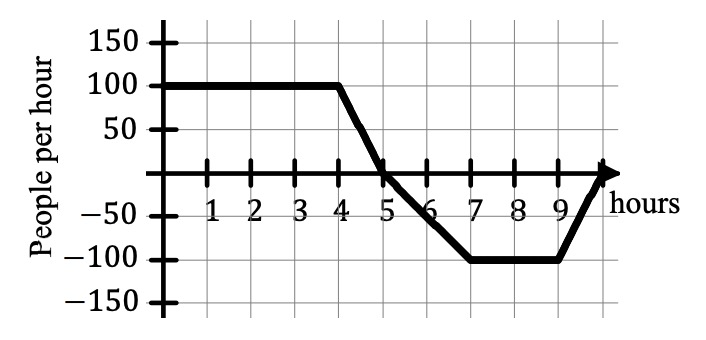
\includegraphics[width=0.35\linewidth]{Example_39.jpg} % Adjust the image width as
\end{minipage}
\begin{enumerate}
    \item[a.] How many people are in the museum after 5 hours?
\end{enumerate}
\tcblower
\textbf{Solution:} 
To determine the number of people in the museum after 5 hours, we calculate the total change in the number of people by finding the area under the curve from \( t = 0 \) to \( t = 5 \).


\begin{itemize}
    \item From \( t = 0 \) to \( t = 4 \): The rate is \( 100 \) people per hour. The area is:
    \[
    \text{Area} = 100 \times 4 = 400
    \]
    \item From \( t = 4 \) to \( t = 5 \): The rate is decreasing linearly from \( 100 \) to \( 0 \), forming a triangle. The area is:
    \[
    \text{Area} = \frac{1}{2} \times \text{Base} \times \text{Height} = \frac{1}{2} \times 1 \times 100 = 50
    \]
\end{itemize}
Thus, the total number of people after 5 hours is:
\[
\text{Total people} = 400 + 50 = 450
\]
\end{tcolorbox}

\newpage

\subsection{Approximating Area with Riemann Sums}

\begin{Note}{Approximation of the Area with Riemann Sums}{}
\textbf{Definition:}  
Approximating the area under a curve using \textbf{Riemann sums} involves the following steps:

\begin{itemize}
    \item \textbf{Divide the region:} Split the region under the curve into smaller intervals. Each interval corresponds to a rectangle.
    \item \textbf{Calculate rectangle areas:} Use the function's value at a specific point in each interval (left endpoint, right endpoint, or midpoint) to determine the height of the rectangle.
    \item \textbf{Sum up the areas:} Add the areas of all the rectangles to estimate the total area under the curve.
\end{itemize}

\textbf{Key Idea:}  
Riemann sums are particularly useful when the exact area under a curve is difficult or impossible to compute analytically. By using rectangles to approximate the area, this method simplifies the calculation.

\vspace{0.5cm}
\end{Note}

\subsubsection{Left Riemann Sum}
\begin{mytheorem}{Left Riemann Sum}{}
The height of each rectangle is determined by the function value at the \textbf{left endpoint} of each subinterval. The approximate total area is:
\[
\text{Area}_{\text{Left}} = \Delta x \cdot \left[ f(x_0) + f(x_1) + \dots + f(x_{n-1}) \right],
\]
where:
\[
x_0 = a, \quad x_1 = a + \Delta x, \quad \dots, \quad x_{n-1} = b - \Delta x.
\]

\(\Delta x\)} is the width of each subinterval

\begin{minipage}{\linewidth}
    \centering
    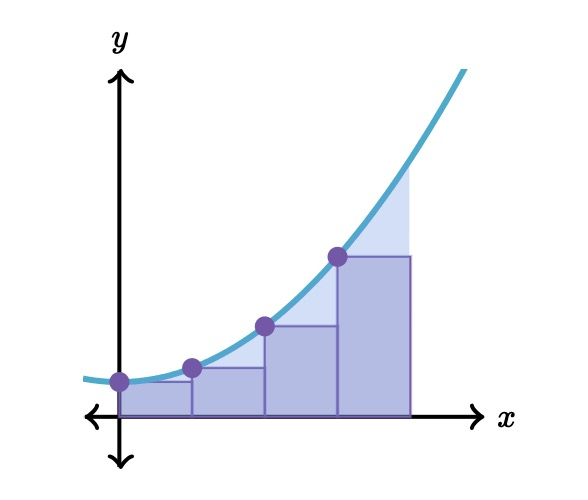
\includegraphics[width=0.35\linewidth]{Example_40.jpg} % Adjust the image width as
\end{minipage}

\end{mytheorem}

\begin{tcolorbox}[colback=examplebg, colframe=red!75!black, title=\textbf{EXAMPLE 1: Use left Riemann Sum to find the Area}, fonttitle=\bfseries, sharp corners]
Given the function:
\[
f(x) = \frac{1}{2}x^3 - x^2 + x + 2
\]
we want to compute the Left Riemann sum on the interval \([1, 3]\) with 4 subintervals.

\begin{minipage}{\linewidth}
    \centering
    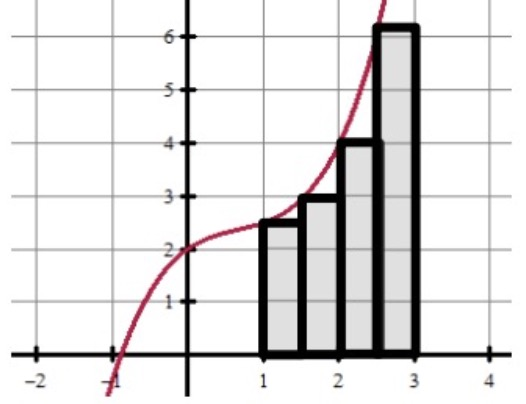
\includegraphics[width=0.40\linewidth]{Example_41.jpg} % Adjust the image width as
\end{minipage}
\tcblower
\textbf{Solution:} 
\textbf{Step 1: Determine \(\Delta x\)}
The width of each subinterval is:
\[
\Delta x = \frac{b-a}{n} = \frac{3-1}{4} = \frac{1}{2}.
\]

\textbf{Step 2: Compute the Left Endpoints}
The left endpoints for the 4 subintervals are:
\[
x_0 = 1, \quad x_1 = 1.5, \quad x_2 = 2, \quad x_3 = 2.5.
\]

\textbf{Step 3: Evaluate \(f(x)\) at Each Left Endpoint}
\[
f(1) = \frac{1}{2}(1)^3 - (1)^2 + 1 + 2 = 2.5,
\]
\[
f(1.5) = \frac{1}{2}(1.5)^3 - (1.5)^2 + 1.5 + 2 = 2.9375,
\]
\[
f(2) = \frac{1}{2}(2)^3 - (2)^2 + 2 + 2 = 4,
\]
\[
f(2.5) = \frac{1}{2}(2.5)^3 - (2.5)^2 + 2.5 + 2 = 6.0625.
\]

\textbf{Step 4: Apply the Left Riemann Sum Formula}
The Left Riemann sum is:
\[
\text{Left Riemann Sum} = \Delta x \left[f(x_0) + f(x_1) + f(x_2) + f(x_3)\right].
\]

Substituting the values:
\[
\text{Left Riemann Sum} = \frac{1}{2} \left[2.5 + 2.9375 + 4 + 6.0625 \right].
\]

Simplify:
\[
\text{Left Riemann Sum} = \frac{1}{2} \cdot 15.5 = 7.75.
\]
\end{tcolorbox}

\subsubsection{Right Riemann Sum}
\begin{mytheorem}{Right Riemann Sum}{}
The height of each rectangle is determined by the function value at the \textbf{right endpoint} of each subinterval. The approximate total area is:
\[
\text{Area}_{\text{Right}} = \Delta x \cdot \left[ f(x_1) + f(x_2) + \dots + f(x_n) \right],
\]
where:
\[
x_1 = a + \Delta x, \quad x_2 = a + 2\Delta x, \quad \dots, \quad x_n = b.
\]

\begin{minipage}{\linewidth}
    \centering
    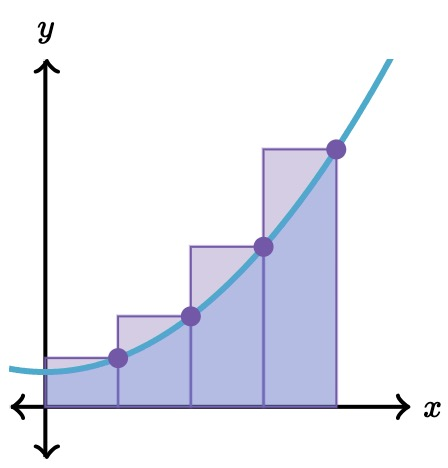
\includegraphics[width=0.25\linewidth]{Example_42.jpg} 
\end{minipage}

    
\end{mytheorem}

\begin{tcolorbox}[colback=examplebg, colframe=red!75!black, title=\textbf{EXAMPLE 2: Use the Right Riemann Sum to Find the Area}, fonttitle=\bfseries, sharp corners]
Given the function:
\[
f(x) = \sqrt{9 - x^2},
\]
we want to compute the Right Riemann sum on the interval \([-2, 1]\) with 3 subintervals.

\begin{minipage}{\linewidth}
    \centering
    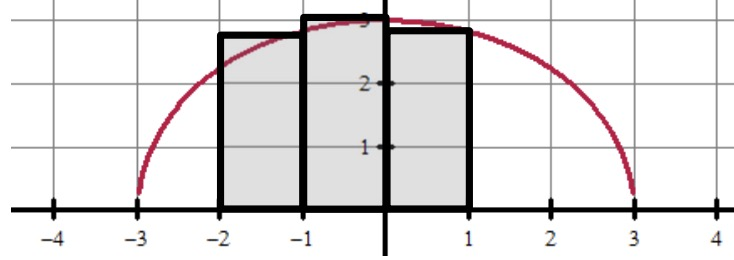
\includegraphics[width=0.35\linewidth]{Example_43.jpg} 
\end{minipage}
\tcblower
\textbf{Solution:} 
\textbf{Step 1: Determine \(\Delta x\)}
The width of each subinterval is:
\[
\Delta x = \frac{b-a}{n} = \frac{1 - (-2)}{3} = \frac{3}{3} = 1.
\]

\textbf{Step 2: Compute the Right Endpoints}
The right endpoints for the 3 subintervals are:
\[
x_1 = -1, \quad x_2 = 0, \quad x_3 = 1.
\]

\textbf{Step 3: Evaluate \(f(x)\) at Each Right Endpoint}
\[
f(-1) =  \sqrt{8},
f(0)  = 3,
f(1)  = \sqrt{8}.
\]


\textbf{Step 4: Apply the Right Riemann Sum Formula}
The Right Riemann sum is:
\[
\text{Right Riemann Sum} = \Delta x \left[f(x_1) + f(x_2) + f(x_3)\right] = 1 \cdot \left[\sqrt{8} + 3 + \sqrt{8} \right] = 8.6568.
\]


\end{tcolorbox}


\subsubsection{Midpoint Riemann Sum}
\begin{mytheorem}{Midpoint Riemann Sum}
The height of each rectangle is determined by the function value at the \textbf{midpoint} of each subinterval. The approximate total area is:
\[
\text{Midpoint Riemann Sum} = \Delta x \cdot \left[f\left(\frac{x_0 + x_1}{2}\right) + f\left(\frac{x_1 + x_2}{2}\right) + \cdots + f\left(\frac{x_{n-1} + x_n}{2}\right)\right],
\]
where \(\frac{x_{i-1} + x_i}{2}\) represents the midpoint of the \(i\)-th subinterval.

\begin{minipage}{\linewidth}
    \centering
    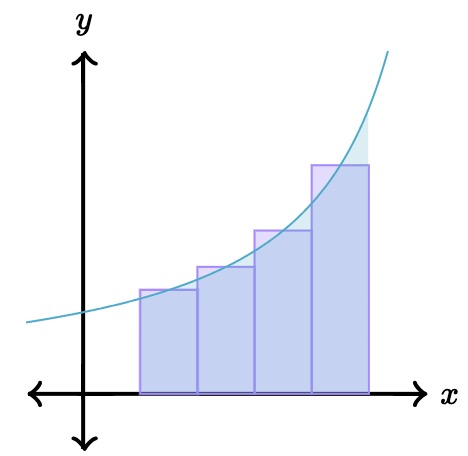
\includegraphics[width=0.30\linewidth]{Example_44.jpg} 
\end{minipage}

\end{mytheorem}


\begin{tcolorbox}[colback=examplebg, colframe=red!75!black, title=\textbf{EXAMPLE 3: Midpoint Rule}, fonttitle=\bfseries, sharp corners]
A rectangular pool gets deeper from one end to the other. The table shows the depth $h(x)$ of the water at 4-foot intervals from one end of the pool to the other.

\begin{center}
\begin{tabular}{|c|c|c|c|c|c|c|c|c|}
\hline
\textbf{Position, $x$ (feet)} & 0 & 4 & 8 & 12 & 16 & 20 & 24  \\
\hline
\textbf{Depth, $h(x)$ (feet)} & 6.5 & 8 & 9.5 & 10 & 11 & 11.5 & 12  \\
\hline
\end{tabular}
\end{center}

 Use a midpoint Riemann Sum with 4 subintervals to approximate the area under the curve from $x = 0$ to $x = 24$.
\tcblower
\textbf{Solution:} 
To approximate the area under the curve from $x = 0$ to $x = 24$ using 4 subintervals, we calculate the midpoint of each subinterval:
\[
\text{Subintervals: } [0, 8], [8, 16], [16, 24]
\]
\[
\text{Midpoints: } x = 4, 12, 20
\]

The midpoint Riemann Sum formula is:
\[
\text{Area} = \Delta x \cdot \left[ h(4) + h(12) + h(20)  \right]
\]
where $\Delta x = 8$ (width of each subinterval).

Substituting the given values:
\[
\text{Area} = 8 \cdot \left[ 8 + 10 + 11.5 \right] = 8 \cdot 29.5 = 236 \, \text{feet}^2
\]





\end{tcolorbox}




\subsubsection{Trapezoid Rule}
\begin{mytheorem}{Trapezoid Rule}{}
Instead of rectangles, the area is approximated by trapezoids. The formula is:
\[
\text{Trapezoid Rule} = \frac{\Delta x}{2} \cdot \left[f(x_0) + 2f(x_1) + 2f(x_2) + \cdots + 2f(x_{n-1}) + f(x_n)\right].
\]

\begin{minipage}{\linewidth}
    \centering
    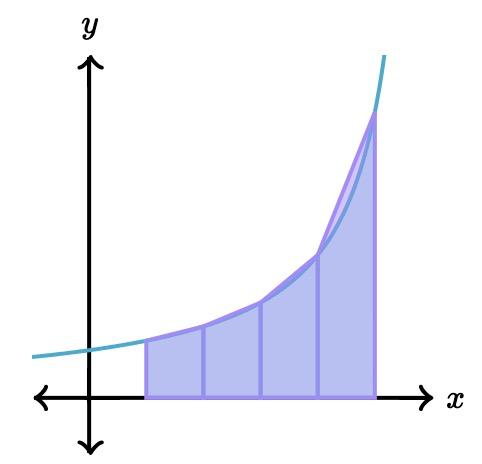
\includegraphics[width=0.30\linewidth]{Example_45.jpg} 
\end{minipage}

\end{mytheorem}

\begin{tcolorbox}[colback=examplebg, colframe=red!75!black, title=\textbf{EXAMPLE 4: Trapezoid Rule}, fonttitle=\bfseries, sharp corners]



The rate at which customers are being served at StarBrusts is given by the continuous function \( R(t) \). A table of selected values of \( R(t) \), for the time interval \( 0 < t \leq 10 \) hours, is shown below. At \( t = 0 \), there had already been 200 customers served.

\begin{center}
\begin{tabular}{|c|c|c|c|c|c|}
\hline
\textbf{Time Hour} & 0 & 2 & 3 & 6 & 10 \\
\hline
\textbf{People/Hour} & 37 & 44 & 36 & 42 & 48\\
\hline
\end{tabular}
\end{center}

Use a trapezoidal sum with four subintervals to approximate how many customers have been served after 10 hours.
\tcblower
\textbf{Solution:} 

The trapezoidal sum formula is:
\[
\text{Area} = \frac{\Delta t}{2} \left[ R(t_1) + 2R(t_2) + 2R(t_3) + \cdots + R(t_n) \right]
\]

From the table, the subinterval widths (\( \Delta t \)) are:
\[
\Delta t_1 = 2, \quad \Delta t_2 = 1, \quad \Delta t_3 = 3, \quad \Delta t_4 = 4
\]

For each subinterval, the trapezoidal sum for the total number of customers served is calculated as:
\[
2 \cdot \frac{37 + 44}{2} + 1 \cdot \frac{44 + 36}{2} + 3 \cdot \frac{36 + 42}{2} + 4 \cdot \frac{42 + 48}{2} =618
\]
\end{tcolorbox}


\subsection{Riemann sums, Summation Notation, and Definite Integral Notation}

\subsubsection{Sigma Notation}
\begin{Definition}{Sigma Notation}{}
    The sum of \( n \) terms \( a_1, a_2, a_3, \dots, a_n \) is written as:
\[
\sum_{i=1}^{n} a_i = a_1 + a_2 + a_3 + \cdots + a_n
\]

\noindent where:
\begin{itemize}
    \item \( i \) is the \textbf{index of summation},
    \item \( a_i \) is the \textbf{\( i \)-th term} of the sum,
    \item The \textbf{upper and lower bounds of summation} are \( n \) and 1, respectively.
\end{itemize}
\end{Definition}

\begin{tcolorbox}[colback=examplebg, colframe=red!75!black, title=\textbf{EXAMPLE 1: Examples of Sigma Notation}, fonttitle=\bfseries, sharp corners]

\begin{enumerate}
    \item[a.] \( \sum_{i=1}^{6} i = 1 + 2 + 3 + 4 + 5 + 6 \)
    
    \item[b.] \( \sum_{i=0}^{5} (i + 1) = 1 + 2 + 3 + 4 + 5 + 6 \)
    
    \item[c.] \( \sum_{j=3}^{7} j^2 = 3^2 + 4^2 + 5^2 + 6^2 + 7^2 \)
    
    \item[d.] \( \sum_{j=1}^{5} \frac{1}{\sqrt{j}} = \frac{1}{\sqrt{1}} + \frac{1}{\sqrt{2}} + \frac{1}{\sqrt{3}} + \frac{1}{\sqrt{4}} + \frac{1}{\sqrt{5}} \)
    
    \item[e.] \( \sum_{k=1}^{n} \frac{1}{n}(k^2 + 1) = \frac{1}{n}(1^2 + 1) + \frac{1}{n}(2^2 + 1) + \cdots + \frac{1}{n}(n^2 + 1) \)
    
    \item[f.] \( \sum_{i=1}^{n} f(x_i) \Delta x = f(x_1) \Delta x + f(x_2) \Delta x + \cdots + f(x_n) \Delta x \)
\end{enumerate}
\end{tcolorbox}


\newpage
\begin{mytheorem}{Summation Formula}{}
 
\begin{enumerate}
    \item \(\sum_{i=1}^n c = cn, \quad c \text{ is a constant.}\)
    \item \(\sum_{i=1}^n i = \frac{n(n+1)}{2}\)
    \item \(\sum_{i=1}^n i^2 = \frac{n(n+1)(2n+1)}{6}\)
    \item \(\sum_{i=1}^n i^3 = \frac{n^2(n+1)^2}{4}\)
\end{enumerate}
   
\end{mytheorem}

\begin{tcolorbox}[colback=examplebg, colframe=red!75!black, title=\textbf{EXAMPLE 2: Evaluating a Sum}, fonttitle=\bfseries, sharp corners]


Evaluate
\[
\sum_{i=1}^n \frac{i+1}{n^2} \quad \text{for } n = 10, 100, 1000, \text{ and } 10,000.
\]




Evaluate
\[
\sum_{i=1}^n \frac{i+1}{n^2} \quad \text{for } n = 10, 100, 1000, \text{ and } 10,000.
\]


\tcblower

\textbf{Solution}

\[
\sum_{i=1}^n \frac{i+1}{n^2} = \frac{1}{n^2} \sum_{i=1}^n (i+1) \quad \text{\textcolor{magenta}{Factor the constant \( 1/n^2 \) out of sum.}}
\]

\[
= \frac{1}{n^2} \left( \sum_{i=1}^n i + \sum_{i=1}^n 1 \right) \quad \text{\textcolor{magenta}{Write as two sums.}}
\]

\[
= \frac{1}{n^2} \left[ \frac{n(n+1)}{2} + n \right] \quad \text{\textcolor{magenta}{Apply Theorem 4.2.}}
\]

\[
= \frac{1}{n^2} \left[ \frac{n^2 + 3n}{2} \right] \quad \text{\textcolor{magenta}{Simplify.}}
\]

\[
= \frac{n + 3}{2n} \quad \text{\textcolor{magenta}{Simplify.}}
\]

\end{tcolorbox}

\newpage
\subsubsection{Riemann Sum}
\begin{tcolorbox}[colback=examplebg, colframe=red!75!black, title=\textbf{EXAMPLE 3: Approximating Area with Riemann Sums }, fonttitle=\bfseries, sharp corners]
Find the area of the region bounded by \( f(x) = e^x \), \( x = 1 \), \( x = 3 \), and the x-axis using a right Riemann sum with 4 subdivisions. Write the right Riemann sum \( A_{\text{Right}} \) with 4 subdivisions using summation notation.

\begin{minipage}{\linewidth}
    \centering
    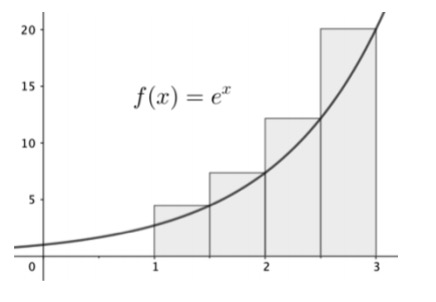
\includegraphics[width=0.30\linewidth]{Example_46.jpg} 
\end{minipage}
\tcblower
\textbf{Solution:} 


   The right Riemann sum is given by:
   \[
   A_{\text{Right}} = \sum_{i=1}^{4} f(x_i) \Delta x = f(1.5)(0.5) + f(2.0)(0.5) + f(2.5)(0.5) + f(3.0)(0.5) = 22.0694
   \]





\end{tcolorbox}
In section 6.2 We have seen the Approximation of the Area with Riemann Sums. Do you know what is the definition of the Riemann Sums?

\begin{Definition}{Riemann Sums}{}
Let $f$ be defined on the closed interval $[a, b]$, and let $\Delta$ be a partition of $[a, b]$ given by
\[
a = x_0 < x_1 < x_2 < \cdots < x_{n-1} < x_n = b,
\]
where $\Delta x_i$ is the width of the $i$th subinterval 
\[
[x_{i-1}, x_i].
\]
If $c_i$ is \textit{any} point in the $i$th subinterval, then the sum
\[
\sum_{i=1}^n f(c_i) \Delta x_i, \quad x_{i-1} \leq c_i \leq x_i
\]
is called a \textbf{Riemann sum} of $f$ for the partition $\Delta$
    
\end{Definition}



\begin{tcolorbox}[colback=examplebg, colframe=red!75!black, title=\textbf{EXAMPLE 4: Finding Upper and Lower Sums for a Region}, fonttitle=\bfseries, sharp corners]
Find the upper and lower sums for the region bounded by the graph of \( f(x) = x^2 \) and the x-axis between \( x = 0 \) and \( x = 2 \).

\tcblower
\textbf{Solution:} 
To begin, partition the interval \([0, 2]\) into \( n \) subintervals, each of width
\[
\Delta x = \frac{b-a}{n} = \frac{2-0}{n} = \frac{2}{n}.
\]

\noindent Using the endpoints of the subintervals:
\begin{itemize}
    \item The left endpoints are \( m_i = 0 + (i-1)\left(\frac{2}{n}\right) = \frac{2(i-1)}{n} \).
    \item The right endpoints are \( M_i = 0 + i\left(\frac{2}{n}\right) = \frac{2i}{n} \).
\end{itemize}

\textbf{Lower Sum:}
Using the left endpoints, the lower sum is
\[
s(n) = \sum_{i=1}^n f(m_i) \Delta x.
\]
Substituting:
\[
s(n) = \sum_{i=1}^n f\left(\frac{2(i-1)}{n}\right)\left(\frac{2}{n}\right),
\]
\[
s(n) = \sum_{i=1}^n \left(\frac{2(i-1)}{n}\right)^2 \cdot \frac{2}{n},
\]



\textbf{Upper Sum:}
Using the right endpoints, the upper sum is
\[
S(n) = \sum_{i=1}^n f(M_i) \Delta x.
\]
Using the right endpoints, the upper sum is
\[
S(n) = \sum_{i=1}^n f(M_i) \Delta x.
\]
Substituting:
\[
S(n) = \sum_{i=1}^n f\left(\frac{2i}{n}\right)\left(\frac{2}{n}\right),
\]
\[
S(n) = \sum_{i=1}^n \left(\frac{2i}{n}\right)^2 \cdot \frac{2}{n},
\]
\end{tcolorbox}

\begin{mytheorem}{Limits of the Lower and Upper Sums}{}
Let \( f \) be continuous and nonnegative on the interval \([a, b]\). The limits as \( n \to \infty \) of both the lower and upper sums exist and are equal to each other. That is,
\[
\lim_{n \to \infty} s(n) = \lim_{n \to \infty} \sum_{i=1}^n f(m_i) \Delta x
\]
\[
= \lim_{n \to \infty} \sum_{i=1}^n f(M_i) \Delta x
\]
\[
= \lim_{n \to \infty} S(n)
\]
where \(\Delta x = \frac{b - a}{n}\) and \(f(m_i)\) and \(f(M_i)\) are the minimum and maximum values of \(f\) on the subinterval.
\end{mytheorem}

\begin{Definition}{Area of a Region in the Plane}{}
    Let \( f \) be continuous and nonnegative on the interval \([a, b]\). The area of the region bounded by the graph of \( f \), the \(x\)-axis, and the vertical lines \(x = a\) and \(x = b\) is given by:
\[
\text{Area} = \lim_{n \to \infty} \sum_{i=1}^n f(c_i) \Delta x
\]
where \(x_{i-1} \leq c_i \leq x_i\) and
\[
\Delta x = \frac{b - a}{n}.
\]

\begin{minipage}{\linewidth}
    \centering
    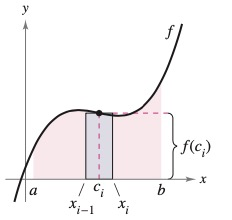
\includegraphics[width=0.40\linewidth]{Example_47.jpg} 
\end{minipage}
\end{Definition}

\begin{tcolorbox}[colback=examplebg, colframe=red!75!black, title=\textbf{EXAMPLE 4: Finding Area by the Limit Definition}, fonttitle=\bfseries, sharp corners]
Find the area of the region bounded by the graph \( f(x) = x^3 \), the \(x\)-axis, and the vertical lines \(x = 0\) and \(x = 1\)

\tcblower
\textbf{Solution:} 
 \(\Delta x = 1/n\), \(c_i = \frac{i}{n}\) 

\[
\text{Area} = \lim_{n \to \infty} \sum_{i=1}^n f(c_i) \Delta x
\]

Substitute \(f(c_i) = \left(\frac{i}{n}\right)^3\) and \(\Delta x = \frac{1}{n}\):
\[
= \lim_{n \to \infty} \sum_{i=1}^n \left(\frac{i}{n}\right)^3 \frac{1}{n}
\]

Simplify:
\[
= \lim_{n \to \infty} \frac{1}{n^4} \sum_{i=1}^n i^3
\]

Apply the formula for the sum of cubes:
\[
= \lim_{n \to \infty} \frac{1}{n^4} \cdot \frac{n^2(n+1)^2}{4}
\]

Simplify further:
\[
= \lim_{n \to \infty} \frac{1}{4} \left( 1 + \frac{1}{n} + \frac{1}{n^2} \right)
\]

As \(n \to \infty\), the terms \(\frac{1}{n}\) and \(\frac{1}{n^2}\) approach 0:
\[
= \frac{1}{4}
\]

Thus, the area of the region is \(\frac{1}{4}\).
\end{tcolorbox}
\newpage
\subsubsection{Definite Integrals}

\begin{Definition}{Definite Integral}{}
If \( f \) is defined on the closed interval \([a, b]\) and the limit of Riemann sums over partitions \(\Delta\) 
\[
\lim_{\|\Delta\| \to 0} \sum_{i=1}^n f(c_i) \Delta x_i
\]
exists (as described above), then \(f\) is said to be \textbf{integrable} on \([a, b]\) and the limit is denoted by
\[
\lim_{\|\Delta\| \to 0} \sum_{i=1}^n f(c_i) \Delta x_i = \int_a^b f(x) \, dx.
\]

The limit is called the \textbf{definite integral} of \(f\) from \(a\) to \(b\). The number \(a\) is the \textbf{lower limit of integration}, and the number \(b\) is the \textbf{upper limit of integration}.
\end{Definition}


\begin{mytheorem}{Continuity Implies Integrability}{}
    If a function \( f \) is continuous on the closed interval \([a, b]\), then \( f \) is integrable on \([a, b]\). That is,
\[
\int_a^b f(x) \, dx \text{ exists.}
\]
\end{mytheorem}


\begin{minipage}{\linewidth}
    \centering
    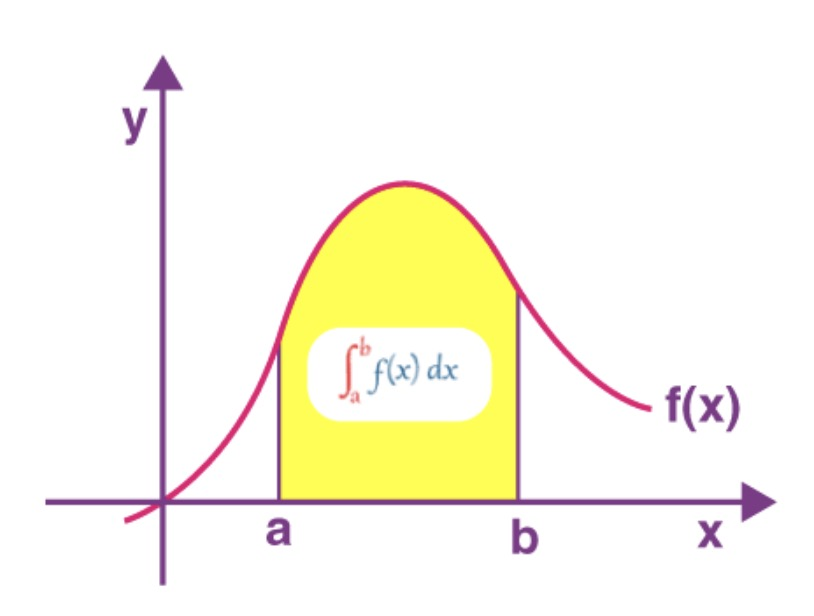
\includegraphics[width=0.75\linewidth]{Example_48.jpg} 
\end{minipage}

\begin{tcolorbox}[colback=examplebg, colframe=red!75!black, title=\textbf{EXAMPLE 5: Evaluating a Definite Integral as a Limit}, fonttitle=\bfseries, sharp corners]
Evaluate the definite integral
\[
\int_{-2}^1 2x \, dx.
\]
\tcblower
\textbf{Solution:} 

Evaluate the definite integral
\[
\int_{-2}^1 2x \, dx.
\]

\noindent\textbf{Solution:} 
\[
\Delta x_i = \Delta x = \frac{b - a}{n} = \frac{3}{n}.
\]

\noindent Choosing \( c_i \) as the right endpoint of each subinterval produces
\[
c_i = a + i(\Delta x) = -2 + \frac{3i}{n}.
\]

\noindent So, the definite integral is
\[
\int_{-2}^1 2x \, dx = \lim_{\|\Delta\| \to 0} \sum_{i=1}^n f(c_i) \Delta x_i.
\]

\noindent Substituting for \( c_i \) and \(\Delta x\), we get:
\[
\int_{-2}^1 2x \, dx = \lim_{n \to \infty} \sum_{i=1}^n f(c_i) \Delta x = \lim_{n \to \infty} \sum_{i=1}^n 2\left(-2 + \frac{3i}{n}\right)\frac{3}{n}.
\]

\noindent Simplify:
\[
\int_{-2}^1 2x \, dx = \lim_{n \to \infty} \frac{6}{n} \sum_{i=1}^n \left(-2 + \frac{3i}{n}\right).
\]

\noindent Split the sum:
\[
\int_{-2}^1 2x \, dx = \lim_{n \to \infty} \frac{6}{n} \left[\sum_{i=1}^n (-2) + \sum_{i=1}^n \frac{3i}{n}\right].
\]

\noindent Use summation formulas:
\[
\int_{-2}^1 2x \, dx = \lim_{n \to \infty} \frac{6}{n} \left[-2n + \frac{3}{n} \sum_{i=1}^n i\right].
\]

\[
\int_{-2}^1 2x \, dx = \lim_{n \to \infty} \frac{6}{n} \left[-2n + \frac{3}{n} \cdot \frac{n(n + 1)}{2}\right].
\]

\noindent Finally:
\[
\int_{-2}^1 2x \, dx = -3.
\]
\end{tcolorbox}


\subsection{The Fundamental Theorem of Calculus and Accumulation Functions (Derivative Part)}

\begin{mytheorem}{}{}
    Define a new function, \( F \), that represents the antiderivative of \( f \):
\[
F(x) = \int_a^x f(t) \, dt
\]

The Fundamental Theorem of Calculus states that if \( f \) is continuous on the interval \((a, b)\), then for every \( x \) in the interval:
\[
\frac{d}{dx} \left[ \int_a^x f(t) \, dt \right] = F'(x) = f(x).
\]
\end{mytheorem}

\begin{tcolorbox}[colback=examplebg, colframe=red!75!black, title=\textbf{EXAMPLE 1:  Fundamental Theorem of Calculus}, fonttitle=\bfseries, sharp corners]
Evaluate 
\[
\frac{d}{dx} \left[ \int_0^x \sqrt{t^2 + 1} \, dt \right].
\]
\tcblower
\textbf{Solution:} 
Note that \( f(t) = \sqrt{t^2 + 1} \) is continuous on the entire real number line. Using the Second Fundamental Theorem of Calculus, you can write:
\[
\frac{d}{dx} \left[ \int_0^x \sqrt{t^2 + 1} \, dt \right] = \sqrt{x^2 + 1}.
\]


\end{tcolorbox}

\newpage

\begin{Note}{Lower Limit of Integration}{}
What happens if the limits of integration are swapped, and the independent variable of the function becomes the lower limit of integration?
\vspace{5mm}
Simply swap the limits and apply a negative sign:

\[
\frac{d}{dx} \int_x^3 \left( 2 - t^2 + t^4 \right) dt = -\frac{d}{dx} \int_3^x \left( 2 - t^2 + t^4 \right) dt.
\]

\end{Note}

\begin{Note}{More Complicated Function of \(x\)}{}
 If there is a more complicated function of \(x\) in the limit of integration, use the chain rule! For example:

\[
\frac{d}{dx} \int_1^{h(x)} f(t) \, dt = f(h(x)) \cdot h'(x).
\]   
\end{Note}


\begin{tcolorbox}[colback=examplebg, colframe=red!75!black, title=\textbf{EXAMPLE 2: Fundamental Theorem of Calculus}, fonttitle=\bfseries, sharp corners]
\[
F(x) = \int_{\pi/2}^{x^3} \cos t \, dt.
\]
\tcblower
\textbf{Solution:} 

\[
\frac{d}{du} \left[ \int_{\pi/2}^u \cos t \, dt \right] = \cos u.
\]

\noindent Therefore:
\[
F'(x) = \cos u \frac{du}{dx}.
\]

\noindent Substitute \( u = x^3 \) and \( \frac{du}{dx} = 3x^2 \):
\[
F'(x) = \cos(x^3)(3x^2).
\]



\end{tcolorbox}


\newpage
\begin{Note}{}{}
If there are functions of \(x\) in both limits of integration, the integral can be rewritten as the difference of two integrals with constant lower limits. For example:

\[
\int_{2x}^{\sin(x)} f(t) \, dt = \int_{2x}^{0} f(t) \, dt + \int_{0}^{\sin(x)} f(t) \, dt.
\]
\end{Note}

\begin{tcolorbox}[colback=examplebg, colframe=red!75!black, title=\textbf{EXAMPLE 4: undamental Theorem of Calculus}, fonttitle=\bfseries, sharp corners]
We are given the function:
\[
h(x) = \int_{3x^2}^{x^3} \sqrt{16 - t^2} \, dt
\]
and asked to find \( h'(1) \).
\tcblower
\textbf{Solution:} 

### Step 1: Apply the Fundamental Theorem of Calculus with the Chain Rule
Using the Fundamental Theorem of Calculus and the chain rule, the derivative of \( h(x) \) is:
\[
h'(x) = \sqrt{16 - (x^3)^2} \cdot \frac{d}{dx}(x^3) - \sqrt{16 - (3x^2)^2} \cdot \frac{d}{dx}(3x^2).
\]

### Step 2: Compute Derivatives of the Limits
\[
\frac{d}{dx}(x^3) = 3x^2, \quad \frac{d}{dx}(3x^2) = 6x.
\]

Thus,
\[
h'(x) = \sqrt{16 - x^6} \cdot 3x^2 - \sqrt{16 - 9x^4} \cdot 6x.
\]

### Step 3: Evaluate \( h'(1) \)
Substitute \( x = 1 \) into the equation:
\[
h'(1) = \sqrt{16 - 1^6} \cdot 3(1)^2 - \sqrt{16 - 9(1)^4} \cdot 6(1).
\]

Simplify each term:
\[
h'(1) = \sqrt{16 - 1} \cdot 3 - \sqrt{16 - 9} \cdot 6,
\]
\[
h'(1) = \sqrt{15} \cdot 3 - \sqrt{7} \cdot 6.
\]

### Final Answer:
\[
h'(1) = 3\sqrt{15} - 6\sqrt{7}.
\]




\end{tcolorbox}


\newpage
\subsection{Behavior of Accumulation Function Involving Area}

For this chapter, we'll focus on graphical, numerical, analytical, and verbal representations to gain a comprehensive understanding of integrally-defined functions
\begin{Note}{Fundamental Theorem of Calculus}{}
Use that derivative to analyze the behavior of such functions. In all cases, the key step will be applying the Fundamental Theorem of Calculus (FTC) to calculate a derivative.
\[
F(n) = \int_a^n f(x) \, dt
\]
Then,
\[
F'(n) = f(x)
\]
\end{Note}

\begin{minipage}{\linewidth}
    \centering
    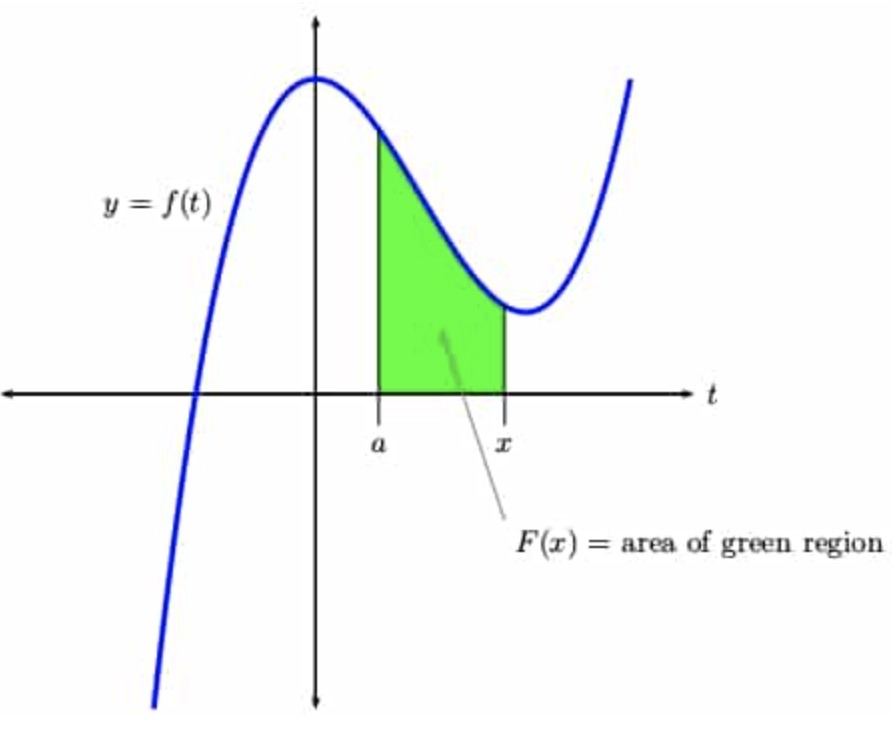
\includegraphics[width=0.50\linewidth]{Example_50.jpg} 
\end{minipage}


\[
\frac{d}{dx} \left[ \int_a^x f(t) \, dt \right] = F'(x) = f(x).
\]

\textbf{Before doing the practice, let us review some important knowledge in derivative}

\begin{table}[h!]
\centering
\begin{tabular}{|l|c|c|}
\hline
\textbf{If $F(x)$ is...} & \textbf{then $F'(x)$} & \textbf{and $F''(x)$} \\ \hline
Increasing              & $+$                   & ---                   \\ \hline
Decreasing              & $-$                   & ---                   \\ \hline
Relative Maximum        & $0$ and changes from $+$ to $-$ & is $-$           \\ \hline
Relative Minimum        & $0$ and changes from $-$ to $+$ & is $+$           \\ \hline
Concave Up              & ---                   & is $+$                \\ \hline
Concave Down            & ---                   & is $-$                \\ \hline
Inflection Point        & ---                   & Changes Sign          \\ \hline
\end{tabular}
\caption{Quick Refresher Chart}
\end{table}


\begin{tcolorbox}[colback=examplebg, colframe=red!75!black, title=\textbf{EXAMPLE 1: FCT}, fonttitle=\bfseries, sharp corners]

\begin{minipage}{\linewidth}
    \centering
    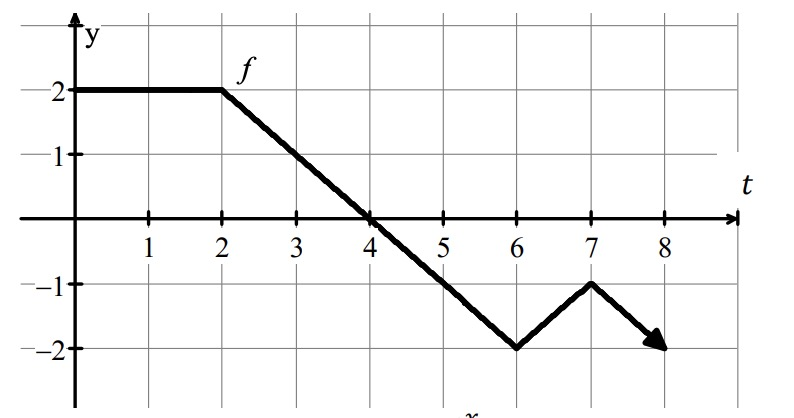
\includegraphics[width=0.40\linewidth]{Example_49.jpg} 
\end{minipage}

\vspace{3mm}

The graph of the function $f$ is shown above. Let 
\[
g(x) = \int_0^x f(t) \, dt.
\]
\begin{enumerate}
    \item[(a)] Find the value of $g'(6)$.
    \item[(b)] Find the value of $g''(6)$.
\end{enumerate}
\tcblower
\textbf{Solution:} 
\begin{enumerate}
    \item[(a)] Using the Fundamental Theorem of Calculus, $g'(x) = f(x)$. Therefore,
    \[
    g'(6) = f(6) = -2.
    \]

    \item[(b)] To find $g''(6)$, we calculate $f'(6)$. However, the graph of $f$ has a corner at $t = 6$, so $f'(6)$ does not exist. Thus,
    \[
    g''(6) = f'(6) \text{ does not exist.}
    \]
\end{enumerate}


\end{tcolorbox}

\vspace{15mm}

\begin{minipage}{\linewidth}
    \centering
    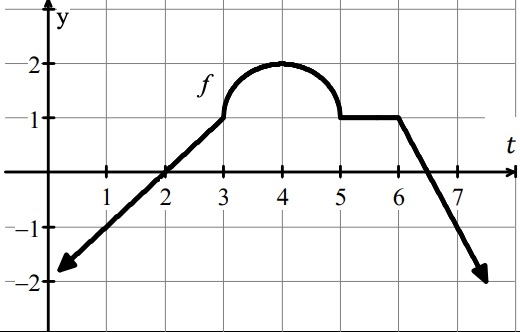
\includegraphics[width=0.70\linewidth]{Example_51.jpg} 
    \label{fig:Example 2}
\end{minipage}

\newpage

\begin{tcolorbox}[colback=examplebg, colframe=red!75!black, title=\textbf{EXAMPLE 2: FCT}, fonttitle=\bfseries, sharp corners]
Let 
\[
g(x) = \int_a^x f(t) \, dt
\]
where the graph of $f$ is shown above and $a$ is a constant. Find the $x$-values of $g$ regarding each of the following conditions:

\begin{enumerate}
    \item[(a)] Relative minimum(s) and maximum(s)
    \item[(b)] Intervals where $g$ is concave up or concave down
    \item[(c)] Intervals where $g$ is increasing or decreasing
    \item[(d)] Point(s) of inflection
    \item[(e)] If $g(3) = -2$, what is the maximum value of $g$ on the interval $[3, 7]$?
    \item[(f)] Given 
    \[
    h(x) = \int_0^{2x-7} f(t) \, dt,
    \]
    find the $x$-value where $h$ has a relative minimum.
\end{enumerate}

\tcblower
\textbf{Solution:} 
\begin{enumerate}
    \item[(a)] Relative minimum at $x = 2$, and maximum at $x = 6.5$.
    \item[(b)] $g$ is concave up on $(-\infty, 4)$ and concave down on $(4, 5) \cup (6, \infty)$.
    \item[(c)] $g$ is increasing on $(2, 6.5)$, and decreasing on $(-\infty, 2) \cup (6.5, \infty)$
    \item[(d)] Point of inflection at $x = 4$.
    \item[(e)] Using the given value $g(3) = -2$:
    \[
    g(6.5) = g(3) + \int_3^{6.5} f(t) \, dt = -2 + \left( 5 + 2 + \frac{1}{4} \right) = \frac{5}{4} + 7 = \frac{33}{4}.
    \]
    Thus, the maximum value of $g$ on $[3, 7]$ is $\frac{33}{4}$.
    \item[(i)] Differentiating $h(x)$:
    \[
    h'(x) = f(2x-7) \cdot 2.
    \]
    Setting $h'(x) = 0$:
    \[
    f(2x-7) = 0 \implies 2x-7 = 2 \implies x = \frac{9}{2}.
    \]
    Thus, $h$ has a relative minimum at $x = \frac{9}{2}$.
\end{enumerate}
\end{tcolorbox}


\newpage

\subsection{Properties of Definite Integrals}
\begin{Definition}{Definite Integral}{}
Integrating a given function over the given interval $[a, b]$ to get a value, or to find the area under $f(x)$ on $[a, b]$.

\[
\int_a^b f(x) \, dx
\]


\begin{itemize}
    \item The $b$ is the \textbf{upper limit of integration}, so it will always be the larger number in the given interval.
    \item The $a$ is the \textbf{lower limit of integration}, so it will be the smaller number in the given interval.
    \item $f(x)$ is the \textbf{function} that we are integrating with respect to $x$.
\end{itemize}
    
\end{Definition}
There are many definitive integral properties that you should memorize.

\begin{mytheorem}{Two Special Definite Integrals}{}
    \begin{enumerate}
    \item If $f$ is defined at $x = a$, then
    \[
    \int_a^a f(x) \, dx = 0.
    \]
    
    \item If $f$ is integrable on $[a, b]$, then
    \[
    \int_a^b f(x) \, dx = -\int_b^a f(x) \, dx.
    \]
\end{enumerate}
\end{mytheorem}


\begin{mytheorem}{Additive Interval Property}{}
    If $f$ is integrable on the three closed intervals determined by $a$, $b$, and $c$, then
\[
\int_a^b f(x) \, dx = \int_a^c f(x) \, dx + \int_c^b f(x) \, dx.
\]
\end{mytheorem}



\begin{mytheorem}{Properties of Definite Integrals}{}
    If $f$ and $g$ are integrable on $[a, b]$ and $k$ is a constant, then the functions $kf$ and $f \pm g$ are integrable on $[a, b]$, and
\begin{enumerate}
    \item $\int_a^b kf(x) \, dx = k \int_a^b f(x) \, dx$
    \item $\int_a^b \big(f(x) \pm g(x)\big) \, dx = \int_a^b f(x) \, dx \pm \int_a^b g(x) \, dx.$
\end{enumerate}
\end{mytheorem}



\begin{tcolorbox}[colback=examplebg, colframe=red!75!black, title=\textbf{EXAMPLE 1: Find the Integral}, fonttitle=\bfseries, sharp corners]
Let $f$ and $g$ be continuous functions that produce the following definite integral values:
\[
\int_{-3}^{2} f(x) \, dx = 2, \quad \int_{2}^{7} f(x) \, dx = -5, \quad \int_{-3}^{2} g(x) \, dx = 6.
\]

Find the following:

\begin{enumerate}
    \item[5.] $\int_{2}^{7} 2f(x) \, dx$
    \item[6.] $4 \int_{-3}^{2} f(x) \, dx$
    \item[7.] $\int_{-3}^{7} f(x) \, dx$
    \item[8.] $\int_{-3}^{2} g(x) \, dx$
    \item[9.] $\int_{-3}^{2} [g(x) - f(x)] \, dx$
    \item[10.] $\left|\int_{2}^{7} f(x) \, dx\right|$
    \item[11.] $-\int_{7}^{2} f(x) \, dx$
\end{enumerate}



\tcblower
\textbf{Solution:} 
\begin{enumerate}
    \item[5.] $\int_{2}^{7} 2f(x) \, dx = -10$
    \item[6.] $4 \int_{-3}^{2} f(x) \, dx = 8$
    \item[7.] $\int_{-3}^{7} f(x) \, dx = 2 + (-5) = -3$
    \item[8.] $\int_{-3}^{2} g(x) \, dx = -6$
    \item[9.] $\int_{-3}^{2} [g(x) - f(x)] \, dx = 6 - 2 = 4$
    \item[10.] $\left|\int_{2}^{7} f(x) \, dx\right| = 5$
    \item[11.] $-\int_{7}^{2} f(x) \, dx = -(-5) = -5$
\end{enumerate}



\end{tcolorbox}


\begin{tcolorbox}[colback=examplebg, colframe=red!75!black, title=\textbf{EXAMPLE 2: Find the Integral}, fonttitle=\bfseries, sharp corners]
\begin{minipage}{\linewidth}
    \centering
    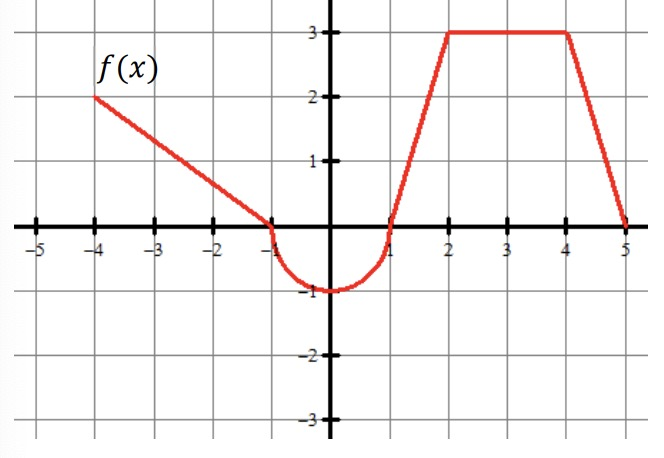
\includegraphics[width=0.55\linewidth]{Example_52.jpg} 
\end{minipage}
\begin{enumerate}
    \item $\int_{-4}^{-1} f(x) \, dx$
    \item $\int_{1}^{2} f(x) \, dx$
    \item $\int_{1}^{5} 2f(x) \, dx$
    \item $\int_{4}^{5} f(x) \, dx$
    \item $\int_{2}^{4} f(x) \, dx$
    \item $\int_{-1}^{4} |f(x)| \, dx$
\end{enumerate}




\tcblower
\textbf{Solution:} 
\begin{enumerate}
    \item $\int_{-4}^{-1} f(x) \, dx = 3$
    \item $\int_{1}^{2} f(x) \, dx = -1.5$
    \item $\int_{1}^{5} 2f(x) \, dx = 18$
    \item $\int_{4}^{5} f(x) \, dx = 12 - \frac{\pi}{2}$
    \item $\int_{2}^{4} f(x) \, dx = -6$
    \item $\int_{-1}^{4} |f(x)| \, dx = 3 + \frac{\pi}{2}$
\end{enumerate}



\end{tcolorbox}


\newpage 

\begin{tcolorbox}[colback=examplebg, colframe=red!75!black, title=\textbf{EXAMPLE 3: Find the Integral}, fonttitle=\bfseries, sharp corners]
If 
\[
\int_1^5 f(x) \, dx = 3, \quad \int_5^{10} f(x) \, dx = 5, \quad \text{and} \quad \int_{10}^{13} f(x) \, dx = -7,
\]
find 
\[
\int_1^{13} f(x) \, dx.
\]


\tcblower
\textbf{Solution:} 

Using the additive interval property, we have:
\[
\int_1^{13} f(x) \, dx = \int_1^5 f(x) \, dx + \int_5^{10} f(x) \, dx + \int_{10}^{13} f(x) \, dx.
\]

Substituting the given values:
\[
\int_1^{13} f(x) \, dx = 3 + 5 - 7.
\]

Simplifying:
\[
\int_1^{13} f(x) \, dx = 1.
\]
\end{tcolorbox}


\newpage
\subsection{The Fundamental Theorem of Calculus and Definite Integrals}
\subsubsection{ Fundamental Theorem of Calculus Part 1}

\begin{mytheorem}{Fundamental Theorem of Calculus Part 1 }{}
    
The first part of the Fundamental Theorem of Calculus (FTOC) states the relationship between antiderivatives and definite integrals. 
\[
g(x) = \int_a^x f(t) \, dt
\]
\[
g'(x) = f(x)
\]

\begin{minipage}{\linewidth}
    \centering
    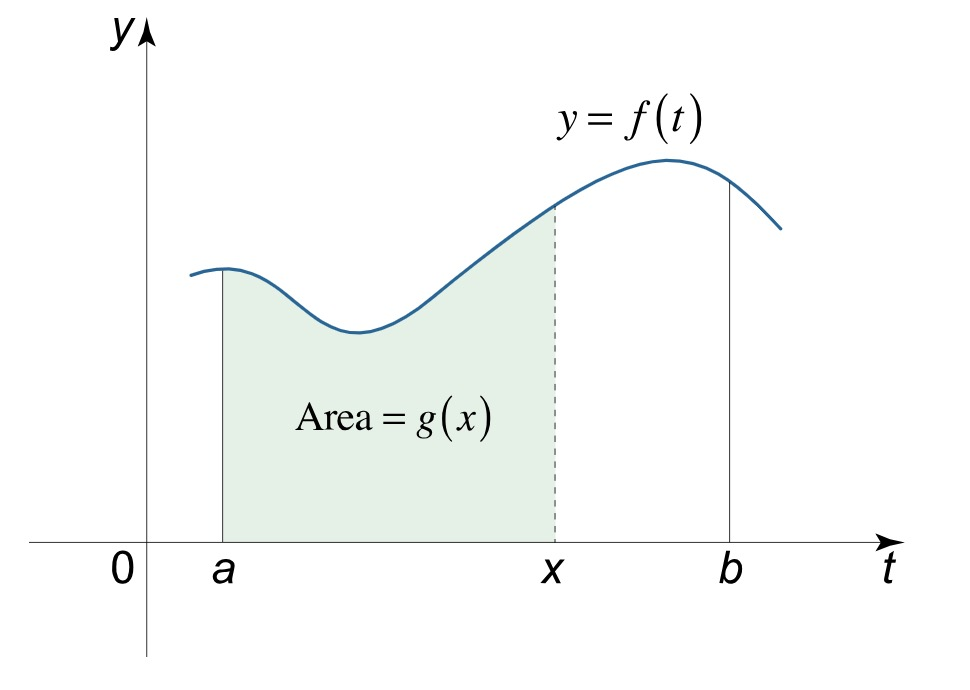
\includegraphics[width=0.55\linewidth]{Example_53.jpg} 
\end{minipage}
\end{mytheorem}

\newpage

\subsubsection{Fundamental Theorem of Calculus - Part 2}
\begin{mytheorem}{Fundamental Theorem of Calculus-Integral}{}
The second part of the Fundamental Theorem of Calculus (FTOC) is more frequently used to solve definite integrals. If a function is continuous on the interval $[a, b]$ and $F$ is an antiderivative of $f$, then
\[
\int_a^b f(x) \, dx = F(b) - F(a).
\]   
\end{mytheorem}

\begin{tcolorbox}[colback=examplebg, colframe=red!75!black, title=\textbf{EXAMPLE 1: Find the Integral of the Function}, fonttitle=\bfseries, sharp corners]
The graph of $f$ is shown in the figure to the right. If 
\[
\int_0^3 f(x) \, dx = 3.5 \quad \text{and} \quad F'(x) = f(x),
\]
then $F(4) - F(0)$ is:

\begin{minipage}{\linewidth}
    \centering
    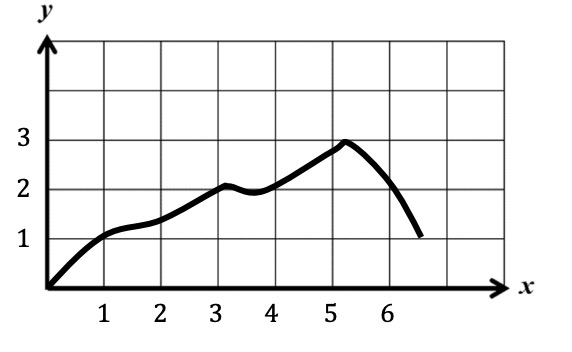
\includegraphics[width=0.55\linewidth]{Example_54.jpg} 
\end{minipage}
\tcblower
\textbf{Solution:} 
\[
F(4) - F(0) = \int_0^4 f(x) \, dx
\]

Using the additive property of integrals:
\[
\int_0^4 f(x) \, dx = \int_0^3 f(x) \, dx + \int_3^4 f(x) \, dx.
\]

From the graph:
\[
\int_0^3 f(x) \, dx = 3.5, \quad \int_3^4 f(x) \, dx = 2.
\]

Thus:
\[
\int_0^4 f(x) \, dx = 3.5 + 2 = 5.5.
\]




\end{tcolorbox}


\newpage
\begin{tcolorbox}[colback=examplebg, colframe=red!75!black, title=\textbf{EXAMPLE 2: Find the Integral of the Function}, fonttitle=\bfseries, sharp corners]
\begin{enumerate}
    \item $\int_0^4 (2x + 4) \, dx$
    \item $\int_0^{\pi/2} (\sin x - x) \, dx$
    \item $\int_{-1}^3 (6x^2 - 8) \, dx$
    \item $\int_4^9 \frac{1}{\sqrt{x}} \, dx$
\end{enumerate}



\tcblower
\textbf{Solution:} 
\begin{enumerate}
    \item $\int_0^4 (2x + 4) \, dx$
    \[
    \frac{2x^2}{2} + 4x \Big|_0^4 = (16 + 16) - (0) = 32
    \]

    \item $\int_0^{\pi/2} (\sin x - x) \, dx$
    \[
    -\cos x - \frac{x^2}{2} \Big|_0^{\pi/2} = \Big[-\cos\left(\frac{\pi}{2}\right) - \frac{\pi^2}{8}\Big] - \Big[ - \cos(0) - 0\Big] = 1 - \frac{\pi^2}{8}
    \]

    \item $\int_{-1}^3 (6x^2 - 8) \, dx$
    \[
    \frac{6x^3}{3} - 8x \Big|_{-1}^3 = \Big[(2 \cdot 27) - 24\Big] - \Big[ (2 \cdot -1) + 8\Big] = 24
    \]

    \item $\int_4^9 \frac{1}{\sqrt{x}} \, dx$
    \[
    2\sqrt{x} \Big|_4^9 = 2(3) - 2(2) = 2
    \]

\end{enumerate}
\end{tcolorbox}

\newpage
\subsection{Finding Antiderivatives and Indefinite Integrals}

\subsubsection{The Antiderivative of a Function}
\begin{Definition}{Antiderivative }{}
    A function $F$ is called an \textit{antiderivative} of $f$ on an interval $I$ if 
\[
F'(x) = f(x) \quad \text{for all } x \text{ in } I.
\]
\end{Definition}

let $f(x) = x^2$. It isn’t difficult to discover an antiderivative of $f$ if we keep the Power Rule in mind. In fact, if 
\[
F(x) = \frac{1}{3}x^3, \quad \text{then } F'(x) = x^2 = f(x).
\]
But the function 
\[
G(x) = \frac{1}{3}x^3 + 100 \quad \text{also satisfies } G'(x) = x^2.
\]
Therefore, both $F$ and $G$ are antiderivatives of $f$. Indeed, any function of the form 
\[
H(x) = \frac{1}{3}x^3 + C,
\]
where $C$ is a constant, is an antiderivative of $f$. 

\begin{minipage}{\linewidth}
    \centering
    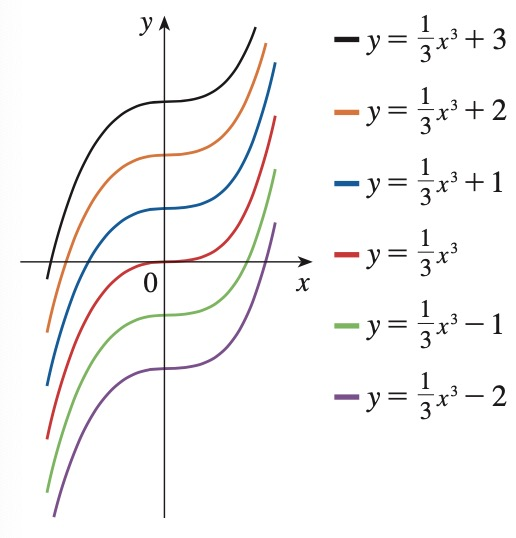
\includegraphics[width=0.45\linewidth]{Example_55.jpg} 
\end{minipage}

\begin{mytheorem}{Antiderivative}{}
If $F$ is an antiderivative of $f$ on an interval $I$, then the most general antiderivative of $f$ on $I$ is
\[
F(x) + C,
\]
where $C$ is an arbitrary constant.
    
\end{mytheorem}

\begin{tcolorbox}[colback=examplebg, colframe=red!75!black, title=\textbf{EXAMPLE 1:Find the most general antiderivative of the functions}, fonttitle=\bfseries, sharp corners]
\begin{enumerate}
    \item $f(x) = \sin x$
    \item $f(x) = \frac{1}{x}$
    \item $f(x) = x^n$, where $n \neq -1$
\end{enumerate}


\tcblower
\textbf{Solution:} 
\begin{enumerate}
    \item For $f(x) = \sin x$:
    \[
    G(x) = -\cos x + C
    \]

    \item For $f(x) = \frac{1}{x}$:
    \[
    G(x) =
    \begin{cases}
    \ln x + C_1, & \text{if } x > 0, \\
    \ln(-x) + C_2, & \text{if } x < 0
    \end{cases}
    \]

    \item For $f(x) = x^n$, where $n \neq -1$:
    \[
    G(x) = \frac{x^{n+1}}{n+1} + C
    \]
\end{enumerate}



\end{tcolorbox}


\newpage
\subsubsection{Antidifferentiation Formulas}

\begin{table}[h!]
\centering
\renewcommand{\arraystretch}{1.5}
\begin{tabular}{|c|c|c|c|}
\hline
\textbf{\textcolor{purple}{Function}} & \textbf{\textcolor{purple}{Particular Antiderivative}} & \textbf{\textcolor{purple}{Function}} & \textbf{\textcolor{purple}{Particular Antiderivative}} \\ \hline
$cf(x)$ & $cF(x)$ & $\sin x$ & $-\cos x$ \\ \hline
$f(x) + g(x)$ & $F(x) + G(x)$ & $\sec^2 x$ & $\tan x$ \\ \hline
$x^n \, (n \neq -1)$ & $\frac{x^{n+1}}{n+1}$ & $\sec x \tan x$ & $\sec x$ \\ \hline
$\frac{1}{x}$ & $\ln |x|$ & $\frac{1}{\sqrt{1 - x^2}}$ & $\sin^{-1} x$ \\ \hline
$e^x$ & $e^x$ & $\frac{1}{1 + x^2}$ & $\tan^{-1} x$ \\ \hline
$b^x$ & $\frac{b^x}{\ln b}$ & $\cosh x$ & $\sinh x$ \\ \hline
$\cos x$ & $\sin x$ & $\sinh x$ & $\cosh x$ \\ \hline
\end{tabular}
\caption{\textcolor{purple}{Table of Antidifferentiation Formulas}}
\end{table}

\begin{tcolorbox}[colback=examplebg, colframe=red!75!black, title=\textbf{EXAMPLE 2: Find the Integral of the Function}, fonttitle=\bfseries, sharp corners]
Find all functions $g$ such that:
\[
g'(x) = 4 \sin x + \frac{2x^5 - \sqrt{x}}{x}.
\]


\tcblower
\textbf{Solution:} 
We first rewrite the given function as follows:
\[
g'(x) = 4 \sin x + \frac{2x^5}{x} - \frac{\sqrt{x}}{x} = 4 \sin x + 2x^4 - x^{-1/2}.
\]

Thus, we want to find an antiderivative of:
\[
g'(x) = 4 \sin x + 2x^4 - x^{-1/2}.
\]

Using the formulas in the Table of Antidifferentiation Formulas and Theorem 1, we obtain:
\[
g(x) = 4(-\cos x) + 2 \cdot \frac{x^5}{5} - \frac{x^{1/2}}{1/2} + C.
\]

Simplifying:
\[
g(x) = -4 \cos x + \frac{2}{5}x^5 - 2\sqrt{x} + C.
\]



\end{tcolorbox}

\begin{tcolorbox}[colback=examplebg, colframe=red!75!black, title=\textbf{EXAMPLE 2: Find the Integral of the Function}, fonttitle=\bfseries, sharp corners]
Find $f$ if $f'(x) = e^x + 20(1 + x^2)^{-1}$ and $f(0) = -2$.


\tcblower
\textbf{Solution:} 

The general antiderivative of $f'(x)$  
is 
\[
f(x) = e^x + 20 \tan^{-1} x + C.
\]

To determine $C$, we use the fact that $f(0) = -2$:
\[
f(0) = e^0 + 20 \tan^{-1} 0 + C = -2.
\]

Simplifying:
\[
1 + 0 + C = -2 \implies C = -3.
\]

Thus, the particular solution is:
\[
f(x) = e^x + 20 \tan^{-1} x - 3.
\]


\end{tcolorbox}


\begin{tcolorbox}[colback=examplebg, colframe=red!75!black, title=\textbf{EXAMPLE 3: Find the Integral of the Function}, fonttitle=\bfseries, sharp corners]

Find $f$ if $f''(x) = 12x^2 + 6x - 4$, $f(0) = 4$, and $f(1) = 1$.

\tcblower
\textbf{Solution:} 
The general antiderivative of 
\[
f''(x) = 12x^2 + 6x - 4
\]
is
\[
f'(x) = \int (12x^2 + 6x - 4) \, dx = \frac{12x^3}{3} + \frac{6x^2}{2} - 4x + C = 4x^3 + 3x^2 - 4x + C.
\]

Using the antidifferentiation rules once more, we find:
\[
f(x) = \int (4x^3 + 3x^2 - 4x + C) \, dx = \frac{4x^4}{4} + \frac{3x^3}{3} - \frac{4x^2}{2} + Cx + D = x^4 + x^3 - 2x^2 + Cx + D.
\]

To determine $C$ and $D$, we use the given conditions:
\begin{itemize}
    \item From $f(0) = 4$, we get $f(0) = 0 + 0 - 0 + 0 + D = 4 \implies D = 4$.
    \item From $f(1) = 1$, we get:  $f(1) = 1 + 1 - 2 + C + 4 = 1 \implies C = -3.$

\end{itemize}

Thus, the required function is:
\[
f(x) = x^4 + x^3 - 2x^2 - 3x + 4.
\]



\end{tcolorbox}


\newpage 
\subsection{Integrating Using Substitution}
\subsubsection{Substitution: Indefinite Integrals}
Because of the Fundamental Theorem, it’s important to be able to find antiderivatives. But our antidifferentiation formulas don’t tell us how to evaluate integrals such as:
\[
\int 2x \sqrt{1 + x^2} \, dx.
\]

To find this integral, we use the problem-solving strategy of \textit{introducing something extra}. 

\begin{mytheorem}{Substitution Rule}{}
    If $u = g(x)$ is a differentiable function whose range is an interval $I$ and $f$ is continuous on $I$, then:
\[
\int f(g(x)) g'(x) \, dx = \int f(u) \, du.
\]
\end{mytheorem}

\begin{tcolorbox}[colback=examplebg, colframe=red!75!black, title=\textbf{EXAMPLE 1: Find the Integral of the Function}, fonttitle=\bfseries, sharp corners]
Find 
\[
\int x^3 \cos(x^4 + 2) \, dx.
\]


\tcblower
\textbf{Solution:} 

We make the substitution $u = x^4 + 2$ because its differential is 
\[
du = 4x^3 \, dx,
\]
which, apart from the constant factor $4$, occurs in the integral. Thus, using 
\[
x^3 \, dx = \frac{1}{4} du
\]
and the Substitution Rule, we have:
\[
\int x^3 \cos(x^4 + 2) \, dx = \int \cos u \cdot \frac{1}{4} du = \frac{1}{4} \int \cos u \, du.
\]

Evaluating the integral:
\[
\frac{1}{4} \int \cos u \, du = \frac{1}{4} \sin u + C.
\]

Substituting back for $u$:
\[
\frac{1}{4} \sin u + C = \frac{1}{4} \sin(x^4 + 2) + C.
\]



\end{tcolorbox}


\begin{tcolorbox}[colback=examplebg, colframe=red!75!black, title=\textbf{EXAMPLE 2: Find the Integral of the Function}, fonttitle=\bfseries, sharp corners]
Find 
\[
\int \sqrt{1 + x^2} \, x^5 \, dx.
\]



\tcblower
\textbf{Solution:} 
An appropriate substitution becomes more apparent if we factor $x^5$ as $x^4 \cdot x$. Let $u = 1 + x^2$. Then $du = 2x \, dx$, so $x \, dx = \frac{1}{2} \, du$. Also, $x^2 = u - 1$, so $x^4 = (u - 1)^2$:

\[
\int \sqrt{1 + x^2} \, x^5 \, dx = \int \sqrt{u} \, (u - 1)^2 \cdot \frac{1}{2} \, du = \frac{1}{2} \int \sqrt{u} \, (u^2 - 2u + 1) \, du.
\]

Simplifying:
\[
\frac{1}{2} \int \sqrt{u} \, (u^2 - 2u + 1) \, du = \frac{1}{2} \int \left(u^{5/2} - 2u^{3/2} + u^{1/2}\right) \, du.
\]

Integrating term by term:
\[
\frac{1}{2} \left( \frac{2}{7}u^{7/2} - \frac{2}{5}u^{5/2} + \frac{2}{3}u^{3/2} \right) + C.
\]

Simplify further:
\[
= \frac{1}{7}(1 + x^2)^{7/2} - \frac{2}{5}(1 + x^2)^{5/2} + \frac{1}{3}(1 + x^2)^{3/2} + C.
\]



\end{tcolorbox}


\begin{tcolorbox}[colback=examplebg, colframe=red!75!black, title=\textbf{EXAMPLE 3: Find the Integral of the Function}, fonttitle=\bfseries, sharp corners]
Evaluate 
\[
\int e^{5x} \, dx.
\]



\tcblower
\textbf{Solution:} 
If we let $u = 5x$, then $du = 5 \, dx$, so $dx = \frac{1}{5} \, du$. Therefore:
\[
\int e^{5x} \, dx = \frac{1}{5} \int e^u \, du.
\]

Integrating:
\[
\frac{1}{5} \int e^u \, du = \frac{1}{5} e^u + C.
\]

Substitute back for $u$:
\[
\frac{1}{5} e^u + C = \frac{1}{5} e^{5x} + C.
\]




\end{tcolorbox}

\begin{tcolorbox}[colback=examplebg, colframe=red!75!black, title=\textbf{EXAMPLE 4: Find the Integral of the Function}, fonttitle=\bfseries, sharp corners]
Evaluate 
\[
\int \tan x \, dx.
\]


\tcblower
\textbf{Solution:} 

First, we write tangent in terms of sine and cosine:
\[
\int \tan x \, dx = \int \frac{\sin x}{\cos x} \, dx.
\]

This suggests that we should substitute $u = \cos x$, since then $du = -\sin x \, dx$ and $\sin x \, dx = -du$:
\[
\int \tan x \, dx = \int \frac{\sin x}{\cos x} \, dx = -\int \frac{1}{u} \, du.
\]

Integrating:
\[
-\int \frac{1}{u} \, du = -\ln |u| + C.
\]

Substitute back for $u$:
\[
-\ln |u| + C = -\ln |\cos x| + C.
\]

Notice that:
\[
-\ln |\cos x| = \ln |\cos x|^{-1} = \ln \frac{1}{|\cos x|} = \ln |\sec x|.
\]

Thus, the result can also be written as:
\[
\int \tan x \, dx = \ln |\sec x| + C.
\]




\end{tcolorbox}



\subsubsection{Substitution: Definite Integrals}
\begin{mytheorem}{Substitution for Definite Integrals}
    If $g'$ is continuous on $[a, b]$ and $f$ is continuous on the range of $u = g(x)$, then:
\[
\int_a^b f(g(x)) g'(x) \, dx = \int_{g(a)}^{g(b)} f(u) \, du.
\]
\end{mytheorem}
\begin{tcolorbox}[colback=examplebg, colframe=red!75!black, title=\textbf{EXAMPLE 5: Changing the Limits of Integration}, fonttitle=\bfseries, sharp corners]
Evaluate 
\[
\int_0^4 \sqrt{2x + 1} \, dx
\]
using the substitution rule.


\tcblower
\textbf{Solution:} 
Using the substitution $u = 2x + 1$, we have $du = 2 \, dx$, so $dx = \frac{1}{2} \, du$. To find the new limits of integration, we note:
\[
\text{When } x = 0, \, u = 2(0) + 1 = 1, \quad \text{and when } x = 4, \, u = 2(4) + 1 = 9.
\]

Therefore:
\[
\int_0^4 \sqrt{2x + 1} \, dx = \int_1^9 \frac{1}{2} \sqrt{u} \, du = \frac{1}{2} \int_1^9 u^{1/2} \, du.
\]

Integrating:
\[
\frac{1}{2} \int_1^9 u^{1/2} \, du = \frac{1}{2} \cdot \frac{2}{3} u^{3/2} \Big|_1^9 = \frac{1}{3} \left( 9^{3/2} - 1^{3/2} \right).
\]

Simplifying:
\[
\frac{1}{3} \left( 9^{3/2} - 1^{3/2} \right) = \frac{1}{3} \left( 27 - 1 \right) = \frac{26}{3}.
\]




\end{tcolorbox}





\begin{tcolorbox}[colback=examplebg, colframe=red!75!black, title=\textbf{EXAMPLE 6: Find the Integral of the Function}, fonttitle=\bfseries, sharp corners]
Evaluate 
\[
\int_1^2 \frac{dx}{(3 - 5x)^2}.
\]


\tcblower
\textbf{Solution:} 
Let $u = 3 - 5x$. Then $du = -5 \, dx$, so $dx = -\frac{1}{5} \, du$. When $x = 1$, $u = 3 - 5(1) = -2$, and when $x = 2$, $u = 3 - 5(2) = -7$. Thus:
\[
\int_1^2 \frac{dx}{(3 - 5x)^2} = \int_{-2}^{-7} \frac{-1}{5u^2} \, du = -\frac{1}{5} \int_{-2}^{-7} u^{-2} \, du.
\]

Integrating:
\[
-\frac{1}{5} \int_{-2}^{-7} u^{-2} \, du = -\frac{1}{5} \left[ -\frac{1}{u} \right]_{-2}^{-7} = \frac{1}{5} \left[ \frac{1}{-7} - \frac{1}{-2} \right].
\]

Simplifying:
\[
\frac{1}{5} \left[ \frac{1}{-7} - \frac{1}{-2} \right] = \frac{1}{5} \left[ -\frac{1}{7} + \frac{1}{2} \right] = \frac{1}{5} \left( \frac{-2 + 7}{14} \right) = \frac{1}{5} \cdot \frac{5}{14} = \frac{1}{14}.
\]
\end{tcolorbox}


\subsection{Integrating Functions Using Long Division and Completing the Square}
\subsubsection{Integrating Using Long Division}

\begin{Note}{Rational Function}{}
 Rational function has a polynomial in the numerator and the denominator of the function

\begin{itemize}
 \item A good rule of thumb is if the numerator of the rational function is an equal degree or higher than the denominator, long division might be the way to go
\end{itemize}
\end{Note}

\begin{tcolorbox}[colback=examplebg, colframe=red!75!black, title=\textbf{EXAMPLE 1: Use Long Division to Simplify the Function}, fonttitle=\bfseries, sharp corners]
\[
\frac{28x^2 + 33x - 35}{4x + 7}
\]


\tcblower
\textbf{Solution:} 
1. Divide the leading terms:
   \[
   \frac{28x^2}{4x} = 7x.
   \]
2. Multiply:
   \[
   7x(4x + 7) = 28x^2 + 49x.
   \]
3. Subtract:
   \[
   (28x^2 + 33x - 35) - (28x^2 + 49x) = -16x - 35.
   \]
4. Divide the next term:
   \[
   \frac{-16x}{4x} = -4.
   \]
5. Multiply:
   \[
   -4(4x + 7) = -16x - 28.
   \]
6. Subtract:
   \[
   (-16x - 35) - (-16x - 28) = -7.
   \]

Thus, the result of the division is:
\[
\frac{28x^2 + 33x - 35}{4x + 7} = 7x - 4 - \frac{7}{4x + 7}.
\]

\end{tcolorbox}


\begin{tcolorbox}[colback=examplebg, colframe=red!75!black, title=\textbf{EXAMPLE 2: Find the Integral of the Function}, fonttitle=\bfseries, sharp corners]

\[
\int \frac{28x^2 + 33x - 35}{4x + 7} \, dx.
\]

\tcblower
\textbf{Solution:} 
\[
\int \frac{28x^2 + 33x - 35}{4x + 7} \, dx = \int (7x - 4 - \frac{7}{4x + 7}) \, dx.
\]

Now, integrate term by term:
\[
\int (7x - 4 - \frac{7}{4x + 7}) \, dx = \int 7x \, dx - \int 4 \, dx - \int \frac{7}{4x + 7} \, dx.
\]

1. For $\int 7x \, dx$:
\[
\int 7x \, dx = \frac{7x^2}{2}.
\]

2. For $\int 4 \, dx$:
\[
\int 4 \, dx = 4x.
\]

3. For $\int \frac{7}{4x + 7} \, dx$, let $u = 4x + 7$, so $du = 4 \, dx$ and $dx = \frac{1}{4} \, du$:
\[
\int \frac{7}{4x + 7} \, dx = \frac{7}{4} \int \frac{1}{u} \, du = \frac{7}{4} \ln|u| + C = \frac{7}{4} \ln|4x + 7| + C.
\]

Combine the results:
\[
\int \frac{28x^2 + 33x - 35}{4x + 7} \, dx = \frac{7x^2}{2} - 4x - \frac{7}{4} \ln|4x + 7| + C.
\]
\end{tcolorbox}


\newpage
\subsubsection{Integrating Using Complete the Square}
If you come across an integral with a \textbf{quadratic expression} in the integrand, and it's missing a perfect square term, \textbf{completing the square} could be very helpful.

\begin{mytheorem}{Completing the Square Formula}{}
    If 
\[
y = x^2 + bx + c,
\]
then by completing the square, we have:
\[
y = \left(x + \frac{b}{2}\right)^2 + c - \left(\frac{b}{2}\right)^2.
\]

To complete the square:
1. Substitute the values of \(b\) and \(c\).
2. Solve to rewrite the quadratic expression in the completed square form.
\end{mytheorem}

\begin{tcolorbox}[colback=examplebg, colframe=red!75!black, title=\textbf{EXAMPLE 3: Completing the Square}, fonttitle=\bfseries, sharp corners]
Simplify the quadratic expression \( y = x^2 + 6x + 5 \) by completing the square.


\tcblower
\textbf{Solution:} 

1. Start with the given expression:
   \[
   y = x^2 + 6x + 5.
   \]

2. Identify the coefficient of \( x \), which is \( b = 6 \).

3. Take half of \( b \) and square it:
   \[
   \left(\frac{b}{2}\right)^2 = \left(\frac{6}{2}\right)^2 = 3^2 = 9.
   \]

4. Add and subtract \( \left(\frac{b}{2}\right)^2 \) inside the equation to complete the square:
   \[
   y = x^2 + 6x + 9 - 9 + 5.
   \]

5. Group the perfect square trinomial and simplify the constant terms:
   \[
   y = (x + 3)^2 - 4.
   \]

\textbf{Final Answer}
The completed square form of \( y = x^2 + 6x + 5 \) is:
\[
y = (x + 3)^2 - 4.
\]

\end{tcolorbox}

\newpage
By carefully manipulating a quadratic expression—adding and subtracting the appropriate value—you can simplify the integral, making it more manageable. This technique is particularly useful in integrals that result in inverse trigonometric functions.

Such transformations often involve completing the square, allowing the integral to take on a standard form that is easier to evaluate.

\begin{tcolorbox}[colback=examplebg, colframe=red!75!black, title=\textbf{EXAMPLE 4: Find the Integral of the Function}, fonttitle=\bfseries, sharp corners]
Evaluate:
\[
\int \frac{1}{\sqrt{-x^2 - 4x - 3}} \, dx.
\]
\tcblower
\textbf{Solution:} 

1. Rewrite the quadratic expression by completing the square:
   \[
   -\left(x^2 + 4x + 4\right) - 3 + 4 = -\left(x + 2\right)^2 + 1.
   \]

2. Substitute this into the integral:
   \[
   \int \frac{1}{\sqrt{1 - \left(x + 2\right)^2}} \, dx.
   \]

3. Recognize the standard form of the inverse sine function:
   \[
   \int \frac{1}{\sqrt{1 - u^2}} \, du = \sin^{-1}(u) + C.
   \]

4. Final result:
   \[
   \int \frac{1}{\sqrt{-x^2 - 4x - 3}} \, dx = \sin^{-1}(x + 2) + C.
   \]
\end{tcolorbox}

\begin{tcolorbox}[colback=examplebg, colframe=red!75!black, title=\textbf{EXAMPLE 5: Find the Integral of the Function}, fonttitle=\bfseries, sharp corners]
Evaluate:
\[
\int \frac{1}{x^2 - 12x + 37} \, dx.
\]


\tcblower
\textbf{Solution:}

1. Rewrite the quadratic expression by completing the square:
   \[
   x^2 - 12x + 37 = \left(x^2 - 12x + 36\right) + 37 - 36 = \left(x - 6\right)^2 + 1.
   \]

2. Substitute this into the integral:
   \[
   \int \frac{1}{(x - 6)^2 + 1} \, dx.
   \]

3. Recognize the standard form of the inverse tangent function:
   \[
   \int \frac{1}{u^2 + 1} \, du = \tan^{-1}(u) + C.
   \]

4. Final result:
   \[
   \int \frac{1}{x^2 - 12x + 37} \, dx = \tan^{-1}(x - 6) + C.
   \]
\end{tcolorbox}


\begin{tcolorbox}[colback=examplebg, colframe=red!75!black, title=\textbf{EXAMPLE 7: Find the Integral of the Function}, fonttitle=\bfseries, sharp corners]
Evaluate:
\[
\int \frac{16}{x^2 - 6x + 25} \, dx.
\]


\tcblower
\textbf{Solution:} 

1. Rewrite the quadratic expression by completing the square:
   \[
   x^2 - 6x + 25 = \left(x^2 - 6x + 9\right) + 25 - 9 = \left(x - 3\right)^2 + 16.
   \]

2. Factor out 16:
   \[
   \int \frac{16}{x^2 - 6x + 25} \, dx = \int \frac{1}{\frac{\left(x - 3\right)^2}{16} + 1} \cdot \frac{16}{16} \, dx.
   \]

3. Let \( u = \frac{x - 3}{4} \), so \( 4 \, du = dx \).

4. Substitute and recognize the standard form of the inverse tangent:
   \[
   \int \frac{1}{u^2 + 1} \, du = \tan^{-1}(u) + C.
   \]

5. Final result:
   \[
   \int \frac{16}{x^2 - 6x + 25} \, dx = \frac{1}{4} \tan^{-1}\left(\frac{x - 3}{4}\right) + C.
   \]
\end{tcolorbox}
\newpage
\subsection{Integrating Using Integration by Parts}
\begin{Note}{BC ONLY}{}
    This is an AP Calculus BC topic only
\end{Note}

\begin{mytheorem}{Integration by Parts}{}
The formula for Integration by Parts is:
\[
\int u \, v \, dx = u \int v \, dx - \int u' \left(\int v \, dx\right) dx,
\]
where:
\begin{itemize}
    \item \( u \) is the function \( u(x) \),
    \item \( v \) is the function \( v(x) \),
    \item \( u' \) is the derivative of the function \( u(x) \).
\end{itemize}
\end{mytheorem}

Here is the product rule, with \( u \) and \( v \) representing two different functions:
\[
\frac{d}{dx}(uv) = u \cdot v' + v \cdot u'.
\]

If we try to reverse the process, we take the integral of all the terms. It will look like the following:
\[
uv = \int u \cdot v' \, dx + \int v \cdot u' \, dx.
\]

Rearranging the terms, we get the following rule for Integration by Parts:
\[
\int u \, dv = uv - \int v \, du.
\]

\subsection*{Where:}
\begin{itemize}
    \item \( u \) and \( dv \) are selected parts of the integrand.
    \item \( du \) is the derivative of \( u \) with respect to the variable of integration.
    \item \( v \) is the antiderivative (integral) of \( dv \).
\end{itemize}

\begin{Note}{Guidance of Integrating by Part}{}
\begin{enumerate}
    \item \textbf{Select \( u \) and \( dv \) carefully.} Choose the variables in a way that simplifies the integral or makes it easier to integrate! We typically use the \textbf{LIATE} mnemonic to quickly choose \( u \), as it tends to efficiently simplify the integral.
    
    \item \textbf{Differentiate and Integrate.} Compute \( du \) and \( v \) by finding the derivative of \( u \) and the antiderivative of \( dv \).
    
    \item \textbf{Apply the Formula.} Plug the values of \( u \), \( dv \), \( v \), and \( du \) into the Integration by Parts formula:
    \[
    \int u \, dv = uv - \int v \, du.
    \]

    \item \textbf{Evaluate the New Integral.} The resulting integral on the right-hand side, involving \( v \) and \( du \), may still need simplification. Repeat the Integration by Parts process if necessary!
    
    \item \textbf{Solve for the Original Integral.} If you end up with a similar integral on both sides of the equation, solve for the original integral using algebraic manipulation.
\end{enumerate}
\end{Note}

\begin{tcolorbox}[colback=blue!5!white, colframe=blue!75!black, title=\textbf{LIATE Mnemonic}]
The \textbf{LIATE} mnemonic provides a guideline for selecting \( u \):
\begin{itemize}
    \item \textbf{L:} Logarithmic functions
    \item \textbf{I:} Inverse trigonometric functions
    \item \textbf{A:} Algebraic functions
    \item \textbf{T:} Trigonometric functions
    \item \textbf{E:} Exponential functions
\end{itemize}
\end{tcolorbox}


\begin{tcolorbox}[colback=examplebg, colframe=red!75!black, title=\textbf{EXAMPLE 1: Find the Integral of the Function}, fonttitle=\bfseries, sharp corners]
Solve \( \int x \cos(x) \, dx \) Using Integration by Parts


\tcblower
\textbf{Solution:} 

We use the Integration by Parts formula:
\[
\int u \, dv = uv - \int v \, du.
\]

1. Let \( u = x \) and \( dv = \cos(x) \, dx \).
   \[
   u = x \quad \text{and} \quad du = 1 \cdot dx,
   \]
   \[
   dv = \cos(x) \, dx \quad \text{and} \quad v = \sin(x).
   \]

2. Apply the formula:
   \[
   \int x \cos(x) \, dx = u v - \int v \, du.
   \]

   Substituting \( u = x \), \( v = \sin(x) \), and \( du = dx \), we get:
   \[
   \int x \cos(x) \, dx = x \sin(x) - \int \sin(x) \, dx.
   \]

3. Compute the remaining integral:
   \[
   \int \sin(x) \, dx = -\cos(x).
   \]

   Substituting this result:
   \[
   \int x \cos(x) \, dx = x \sin(x) - \big(-\cos(x)\big) + C.
   \]

4. Simplify the expression:
   \[
   \int x \cos(x) \, dx = x \sin(x) + \cos(x) + C.
   \]

\end{tcolorbox}

\begin{tcolorbox}[colback=examplebg, colframe=red!75!black, title=\textbf{EXAMPLE 2: Find the Integral of the Function}, fonttitle=\bfseries, sharp corners]

Solve \( \int x^2 \sin(x) \, dx \) Using Tabular Integration by Parts

\tcblower
\textbf{Solution:} 

Given:
\[
f = x^2 \quad \text{and} \quad g' = \sin(x).
\]

\textbf{Step-by-Step Process (Tabular Integration by Parts):}
1. Differentiate \( f \) repeatedly until it becomes zero:
\[
\begin{aligned}
f &= x^2, & f' &= 2x, & f'' &= 2, & f''' &= 0.
\end{aligned}
\]

2. Integrate \( g' \) repeatedly:
\[
\begin{aligned}
g' &= \sin(x), & g &= -\cos(x), & g &= -\sin(x), & g &= \cos(x).
\end{aligned}
\]

3. Apply the tabular integration rule:
\[
\int x^2 \sin(x) \, dx = 
(-x^2)(\cos(x)) + (2x)(-\sin(x)) + (2)(\cos(x)) + C.
\]

\textbf{Simplify:}
\[
\int x^2 \sin(x) \, dx = 
-x^2 \cos(x) + 2x \sin(x) + 2 \cos(x) + C.
\]
\end{tcolorbox}


\begin{tcolorbox}[colback=examplebg, colframe=red!75!black, title=\textbf{EXAMPLE 3: Find the Integral of the Function}, fonttitle=\bfseries, sharp corners]
Solve \( \int_1^e x^4 \ln(x) \, dx \)


\tcblower
\textbf{Solution:} 

Given:
\[
f = \ln(x), \quad f' = \frac{1}{x}, \quad g = \frac{x^5}{5}.
\]

\textbf{Step 1: Integration by Parts Formula}
Using the formula:
\[
\int u \, dv = uv - \int v \, du,
\]
we have:
\[
\int_1^e x^4 \ln(x) \, dx = \left[\frac{x^5}{5} \ln(x)\right]_1^e - \int_1^e \frac{x^5}{5} \cdot \frac{1}{x} \, dx.
\]

\textbf{Step 2: Simplify the Second Integral}
Simplify:
\[
\int_1^e x^4 \ln(x) \, dx = \left[\frac{x^5}{5} \ln(x)\right]_1^e - \int_1^e \frac{x^4}{5} \, dx.
\]

The second integral becomes:
\[
\int_1^e \frac{x^4}{5} \, dx = \frac{1}{5} \int_1^e x^4 \, dx = \frac{1}{5} \cdot \left[\frac{x^5}{5}\right]_1^e.
\]
\end{tcolorbox}


\newpage

\subsection{Integrating Using Linear Partial Fractions}
\begin{Note}{BC ONLY}{}
    This is an AP Calculus BC topic only
\end{Note}
\begin{mytheorem}{Linear Factor}{}
For each factor of the form $(px + q)^m$, the partial fraction decomposition must include the following sum of $m$ fractions:

\[
\frac{A_1}{px + q} + \frac{A_2}{(px + q)^2} + \cdots + \frac{A_m}{(px + q)^m}
\]
\end{mytheorem}

\begin{tcolorbox}[colback=examplebg, colframe=red!75!black, title=\textbf{EXAMPLE 1: Distinct Linear Factors}, fonttitle=\bfseries, sharp corners]
Write the partial fraction decomposition for
\[
\frac{1}{x^2 - 5x + 6}.
\]


\tcblower
\textbf{Solution:} 

Because $x^2 - 5x + 6 = (x - 3)(x - 2)$, you should include one partial fraction for each factor and write
\[
\frac{1}{x^2 - 5x + 6} = \frac{A}{x - 3} + \frac{B}{x - 2},
\]
Multiplying this equation by the least common denominator $(x - 3)(x - 2)$ 
\[
1 = A(x - 2) + B(x - 3). \quad \text{(Basic equation)}
\]

\textbf{To solve for $A$, let $x = 3$:}
\[
1 = A(3 - 2) + B(3 - 3),
\]
\[
1 = A(1) + B(0),
\]
\[
1 = A. \quad \text{(Let $x = 3$ in basic equation.)}
\]

\textbf{To solve for $B$, let $x = 2$:}
\[
1 = A(2 - 2) + B(2 - 3),
\]
\[
1 = A(0) + B(-1),
\]
\[
-1 = B. \quad \text{(Let $x = 2$ in basic equation.)}
\]

So, the decomposition is
\[
\frac{1}{x^2 - 5x + 6} = \frac{1}{x - 3} - \frac{1}{x - 2},
\]


\end{tcolorbox}
    
\begin{tcolorbox}[colback=examplebg, colframe=red!75!black, title=\textbf{EXAMPLE 2: Find the Integral of the Function}, fonttitle=\bfseries, sharp corners]
Find
\[
\int \frac{5x^2 + 20x + 6}{x^3 + 2x^2 + x} \, dx.
\]


\tcblower
\textbf{Solution:} 

Because
\[
x^3 + 2x^2 + x = x(x^2 + 2x + 1) = x(x + 1)^2,
\]
you should include one fraction for each power of $x$ and $(x + 1)$ and write
\[
\frac{5x^2 + 20x + 6}{x(x + 1)^2} = \frac{A}{x} + \frac{B}{x + 1} + \frac{C}{(x + 1)^2}.
\]

Multiplying by the least common denominator $x(x + 1)^2$ yields the \textbf{basic equation}
\[
5x^2 + 20x + 6 = A(x + 1)^2 + Bx(x + 1) + Cx. \quad \text{(Basic equation)}
\]

To solve for $A$, let $x = 0$. This eliminates the $B$ and $C$ terms and yields
\[
6 = A(1)^2 + 0 + 0,
\]
\[
6 = A.
\]

To solve for $C$, let $x = -1$. This eliminates the $A$ and $B$ terms and yields
\[
5(-1)^2 + 20(-1) + 6 = 0 + 0 - C,
\]
\[
9 = C.
\]

The most convenient choices for $x$ have been used, so to find the value of $B$, you can use any other value of $x$ along with the calculated values of $A$ and $C$. Using $x = 1$, $A = 6$, and $C = 9$ produces
\[
5(1)^2 + 20(1) + 6 = A(4) + B(2) + C,
\]
\[
31 = 6(4) + 2B + 9,
\]
\[
-2 = 2B,
\]
\[
-1 = B.
\]

So, it follows that
\[
\int \frac{5x^2 + 20x + 6}{x(x + 1)^2} \, dx = \int \left( \frac{6}{x} - \frac{1}{x + 1} + \frac{9}{(x + 1)^2} \right) \, dx,
\]
\[
= 6 \ln|x| - \ln|x + 1| + 9 \frac{(x + 1)^{-1}}{-1} + C,
\]
\[
= 6 \ln|x| - \ln|x + 1| - \frac{9}{x + 1} + C.
\]

\end{tcolorbox}

\subsection{Evaluating Improper
Integrals}
\begin{Note}{BC ONLY}{}
    This is an AP Calculus BC topic only
\end{Note}


\subsubsection{Improper Integrals with Infinite Limits of Integration}

\begin{Definition}{Improper Integrals with Infinite Integration Limits}{}
\begin{enumerate}
    \item If $f$ is continuous on the interval $[a, \infty)$, then
    \[
    \int_a^\infty f(x) \, dx = \lim_{b \to \infty} \int_a^b f(x) \, dx.
    \]

    \item If $f$ is continuous on the interval $(-\infty, b]$, then
    \[
    \int_{-\infty}^b f(x) \, dx = \lim_{a \to -\infty} \int_a^b f(x) \, dx.
    \]

    \item If $f$ is continuous on the interval $(-\infty, \infty)$, then
    \[
    \int_{-\infty}^\infty f(x) \, dx = \int_{-\infty}^c f(x) \, dx + \int_c^\infty f(x) \, dx,
    \]
    where $c$ is any real number.
\end{enumerate}

In the first two cases, the \textit{improper integral} \textbf{converges} when the limit exists—otherwise, the \textit{improper integral} \textbf{diverges}. 
\end{Definition}

\begin{tcolorbox}[colback=examplebg, colframe=red!75!black, title=\textbf{EXAMPLE 1: An Improper Integral That Diverges}, fonttitle=\bfseries, sharp corners]
Evaluate
\[
\int_1^\infty \frac{dx}{x}.
\]



\tcblower
\textbf{Solution:} 
\[
\int_1^\infty \frac{dx}{x} = \lim_{b \to \infty} \int_1^b \frac{dx}{x}. \quad \text{(Take limit as $b \to \infty$.)}
\]
\[
= \lim_{b \to \infty} \left[ \ln x \right]_1^b. \quad \text{(Apply Log Rule.)}
\]
\[
= \lim_{b \to \infty} \left( \ln b - 0 \right). \quad \text{(Apply Fundamental Theorem of Calculus.)}
\]
\[
= \infty. \quad \text{(Evaluate limit.)}
\]
\end{tcolorbox}

\begin{tcolorbox}[colback=examplebg, colframe=red!75!black, title=\textbf{EXAMPLE 2: Infinite Upper and Lower Limits of Integration}, fonttitle=\bfseries, sharp corners]
\[
\int_{-\infty}^\infty \frac{e^x}{1 + e^{2x}} \, dx.
\]


\tcblower
\textbf{Solution:} 
Note that the integrand is continuous on $(-\infty, \infty)$. To evaluate the integral, you can break it into two parts, choosing $c = 0$ as a convenient value:
\[
\int_{-\infty}^\infty \frac{e^x}{1 + e^{2x}} \, dx = \int_{-\infty}^0 \frac{e^x}{1 + e^{2x}} \, dx + \int_0^\infty \frac{e^x}{1 + e^{2x}} \, dx.
\]

\[
= \lim_{b \to -\infty} \left[ \arctan e^x \right]_b^0 + \lim_{b \to \infty} \left[ \arctan e^x \right]_0^b.
\]

\[
= \lim_{b \to -\infty} \left( \frac{\pi}{4} - \arctan e^b \right) + \lim_{b \to \infty} \left( \arctan e^b - \frac{\pi}{4} \right).
\]

\[
= \frac{\pi}{4} - 0 + \frac{\pi}{2} - \frac{\pi}{4}.
\]

\[
= \frac{\pi}{2}.
\]

\end{tcolorbox}

\newpage

\subsubsection{Improper Integrals with Infinite Discontinuities}
\begin{Definition}{Improper Integrals with Infinite Discontinuities}{}
    \begin{enumerate}
    \item If $f$ is continuous on the interval $[a, b)$ and has an infinite discontinuity at $b$, then
    \[
    \int_a^b f(x) \, dx = \lim_{c \to b^-} \int_a^c f(x) \, dx.
    \]

    \item If $f$ is continuous on the interval $(a, b]$ and has an infinite discontinuity at $a$, then
    \[
    \int_a^b f(x) \, dx = \lim_{c \to a^+} \int_c^b f(x) \, dx.
    \]

    \item If $f$ is continuous on the interval $[a, b]$, except for some $c$ in $(a, b)$ at which $f$ has an infinite discontinuity, then
    \[
    \int_a^b f(x) \, dx = \int_a^c f(x) \, dx + \int_c^b f(x) \, dx.
    \]
\end{enumerate}

In the first two cases, the \textit{improper integral} \textbf{converges} when the limit exists—otherwise, the \textit{improper integral} \textbf{diverges}.
\end{Definition}

\begin{tcolorbox}[colback=examplebg, colframe=red!75!black, title=\textbf{EXAMPLE 3: An Improper Integral That Diverges}, fonttitle=\bfseries, sharp corners]
Evaluate
\[
\int_0^2 \frac{dx}{x^3}.
\]



\tcblower
\textbf{Solution:} 
Because the integrand has an infinite discontinuity at $x = 0$, you can write
\[
\int_0^2 \frac{dx}{x^3} = \lim_{b \to 0^+} \left[ -\frac{1}{2x^2} \right]_b^2,
\]
\[
= \lim_{b \to 0^+} \left( -\frac{1}{8} + \frac{1}{2b^2} \right),
\]
\[
= \infty.
\]

So, you can conclude that the \textit{improper integral} diverges.
\end{tcolorbox}



\begin{tcolorbox}[colback=examplebg, colframe=red!75!black, title=\textbf{EXAMPLE 4: An Improper Integral with an Interior Discontinuity}, fonttitle=\bfseries, sharp corners]
Evaluate
\[
\int_{-1}^2 \frac{dx}{x^3}.
\]


\tcblower
\textbf{Solution:} 
This integral is \textit{improper} because the integrand has an infinite discontinuity at the interior point $x = 0$, as shown in Figure 8.24. So, you can write
\[
\int_{-1}^2 \frac{dx}{x^3} = \int_{-1}^0 \frac{dx}{x^3} + \int_0^2 \frac{dx}{x^3}.
\]

From previous example, you know that the second integral diverges. So, the original \textit{improper integral} also diverges.

\textbf{Note:} Remember to check for infinite discontinuities at interior points as well as at endpoints when determining whether an integral is \textit{improper}. For instance, if you had not recognized that the integral in Example 8 was \textit{improper}, you would have obtained the incorrect result:
\[
\int_{-1}^2 \frac{dx}{x^3} = \left[ -\frac{1}{2x^2} \right]_{-1}^2 = -\frac{1}{8} + \frac{1}{2} = \frac{3}{8}. \quad \text{(Incorrect evaluation.)}
\]
\end{tcolorbox}



\newpage

\subsection{Selecting Techniques for Antidifferentiation}

\begin{mytheorem}{Power Rule}{}
    The power rule for antiderivatives is a fundamental technique used to find the antiderivative of a function raised to a power. When you have an integral in the form $\int x^n \, dx$, this rule is your go-to method.
\vspace{3mm}
This results in:
\[
\int x^n \, dx = \frac{x^{n+1}}{n+1} + C,
\]
where $C$ is the constant of integration.
\end{mytheorem}

\begin{tcolorbox}[colback=examplebg, colframe=red!75!black, title=\textbf{EXAMPLE 1: Find the Integral of the Function}, fonttitle=\bfseries, sharp corners]
Evaluate:
\[
\int x^3 \, dx.
\]


\tcblower
\textbf{Solution:} 
Using the power rule, we add $1$ to the exponent and divide by the new exponent:
\[
\int x^3 \, dx = \frac{x^{3+1}}{3+1} + C = \frac{x^4}{4} + C.
\]

Thus, the antiderivative is:
\[
\frac{x^4}{4} + C.
\]

\end{tcolorbox}

\begin{mytheorem}{Substitution Rule}{}
    If $u = g(x)$ is a differentiable function whose range is an interval $I$ and $f$ is continuous on $I$, then:
\[
\int f(g(x)) g'(x) \, dx = \int f(u) \, du.
\]


The basic steps for \( u \)-substitution are as follows:
\begin{enumerate}
    \item Choose a suitable \( u \) that simplifies the integral.
    \item Find \( du \) (the derivative of \( u \)) and express \( dx \) in terms of \( du \).
    \item Rewrite the integral in terms of \( u \).
    \item Integrate with respect to \( u \).
    \item Substitute back in terms of \( x \) if necessary.
\end{enumerate}
\end{mytheorem}

\begin{tcolorbox}[colback=examplebg, colframe=red!75!black, title=\textbf{EXAMPLE 2: Find the Integral of the Function}, fonttitle=\bfseries, sharp corners]

Evaluate:
\[
\int \frac{x}{\sqrt{x^2 + 4}} \, dx.
\]

\tcblower
\textbf{Solution:} 

1. **Choose a substitution:**

   Let \( u = x^2 + 4 \). This choice simplifies the term inside the square root.

2. **Find \( du \):**

   Differentiate \( u = x^2 + 4 \):
   \[
   du = 2x \, dx \quad \text{or} \quad \frac{1}{2} du = x \, dx.
   \]

3. **Rewrite the integral:**

   Substitute \( u = x^2 + 4 \) and \( x \, dx = \frac{1}{2} du \):
   \[
   \int \frac{x}{\sqrt{x^2 + 4}} \, dx = \int \frac{1}{\sqrt{u}} \cdot \frac{1}{2} \, du.
   \]

   Simplify:
   \[
   \int \frac{x}{\sqrt{x^2 + 4}} \, dx = \frac{1}{2} \int u^{-1/2} \, du.
   \]

4. **Integrate with respect to \( u \):**

   Use the power rule for integration:
   \[
   \int u^{-1/2} \, du = 2u^{1/2}.
   \]

   Therefore:
   \[
   \frac{1}{2} \int u^{-1/2} \, du = \frac{1}{2} \cdot 2u^{1/2} = u^{1/2}.
   \]

5. **Substitute back in terms of \( x \):**

   Recall \( u = x^2 + 4 \). Substituting back:
   \[
   u^{1/2} = \sqrt{x^2 + 4}.
   \]

   Thus, the solution is:
   \[
   \int \frac{x}{\sqrt{x^2 + 4}} \, dx = \sqrt{x^2 + 4} + C,
   \]

   where \( C \) is the constant of integration.

\end{tcolorbox}


\newpage
\begin{mytheorem}{Trigonometric Functions}{}
    Trigonometric functions, like sine, cosine, and tangent, frequently appear in integrals. Understanding how to handle these functions is crucial. 

Common trigonometric integrals include:
\begin{itemize}
    \item \(\int \sin(x) \, dx = -\cos(x) + C\)
    \item \(\int \cos(x) \, dx = \sin(x) + C\)
    \item \(\int \tan(x) \, dx = -\ln|\cos(x)| + C\)
    \item \(\int \cot(x) \, dx = \ln|\sin(x)| + C\)
    \item \(\int \sec(x) \, dx = \ln|\sec(x) + \tan(x)| + C\)
    \item \(\int \csc(x) \, dx = -\ln|\csc(x) + \cot(x)| + C\)
\end{itemize}
\end{mytheorem}



\begin{mytheorem}{Inverse Trigonometric Functions}{}
Antidifferentiation often involves \textit{inverse trigonometric functions} like arcsin, arccos, and arctan. 

Here are some common inverse trigonometric derivatives:
\begin{itemize}
    \item \(\frac{d}{dx} \left( \sin^{-1}(x) \right) = \frac{1}{\sqrt{1-x^2}}\)
    \item \(\frac{d}{dx} \left( \cos^{-1}(x) \right) = \frac{-1}{\sqrt{1-x^2}}\)
    \item \(\frac{d}{dx} \left( \tan^{-1}(x) \right) = \frac{1}{1+x^2}\)
    \item \(\frac{d}{dx} \left( \cot^{-1}(x) \right) = \frac{-1}{1+x^2}\)
    \item \(\frac{d}{dx} \left( \sec^{-1}(x) \right) = \frac{1}{x\sqrt{x^2-1}}\)
    \item \(\frac{d}{dx} \left( \csc^{-1}(x) \right) = \frac{-1}{x\sqrt{x^2-1}}\)
\end{itemize}
\end{mytheorem}

\begin{mytheorem}{Exponentials and Logarithms}{}

Functions involving exponentials ($e^x$) and natural logarithms ($\ln(x)$) frequently appear in calculus problems. Familiarity with their antiderivatives is necessary for solving such integrals.

\begin{enumerate}
    \item \(\int e^x \, dx = e^x + C\)
    \item \(\int \frac{1}{x} \, dx = \ln|x| + C\)
\end{enumerate}

\end{mytheorem}

\begin{tcolorbox}[colback=examplebg, colframe=red!75!black, title=\textbf{EXAMPLE 3: Find the Integral of the Function}, fonttitle=\bfseries, sharp corners]
Evaluate:
\[
\int 3e^{2x} \, dx.
\]


\tcblower
\textbf{Solution:} 

\begin{enumerate}
    \item Use substitution:
    \[
    \text{Let } u = 2x, \quad \text{so } du = 2 \, dx, \quad dx = \frac{1}{2} \, du.
    \]
    \item Integrate:
    \[
    \frac{3}{2} \int e^u \, du = \frac{3}{2} e^u + C.
    \]
    \item Substitute back \( u = 2x \):
    \[
    \int 3e^{2x} \, dx = \frac{3}{2} e^{2x} + C.
    \]
\end{enumerate}

\end{tcolorbox}


\begin{tcolorbox}[colback=examplebg, colframe=red!75!black, title=\textbf{EXAMPLE 4: Find the Integral of the Function}, fonttitle=\bfseries, sharp corners]

Evaluate:
\[
\int \frac{\ln(x)}{x} \, dx.
\]

\tcblower
\textbf{Solution:} 
\begin{enumerate}
    \item Recognize that this integral is suitable for substitution:
    \[
    \text{Let } u = \ln(x), \quad \text{so } du = \frac{1}{x} \, dx.
    \]
    \item Rewrite the integral:
    \[
    \int \frac{\ln(x)}{x} \, dx = \int u \, du.
    \]
    \item Integrate:
    \[
    \int u \, du = \frac{u^2}{2} + C.
    \]
    \item Substitute back \( u = \ln(x) \):
    \[
    \int \frac{\ln(x)}{x} \, dx = \frac{\ln^2(x)}{2} + C.
    \]
\end{enumerate}
\end{tcolorbox}


\newpage

\begin{mytheorem}{Completing the Square Formula}{}
    If 
\[
y = x^2 + bx + c,
\]
then by completing the square, we have:
\[
y = \left(x + \frac{b}{2}\right)^2 + c - \left(\frac{b}{2}\right)^2.
\]
\end{mytheorem}


\begin{tcolorbox}[colback=examplebg, colframe=red!75!black, title=\textbf{EXAMPLE 5: Find the Integral of the Function}, fonttitle=\bfseries, sharp corners]
Evaluate:
\[
\int (x^2 + 4x + 4) \, dx.
\]


\tcblower
\textbf{Solution:} 
\textbf{Step 1: Rewrite the Integral}  
Rewrite the integral using the perfect square trinomial:
\[
\int (x^2 + 4x + 4) \, dx = \int (x + 2)^2 \, dx.
\]

\textbf{Step 2: Use the Power Rule for Antiderivatives}  
Apply the power rule for antiderivatives to find the integral:
\[
\int (x + 2)^2 \, dx = \frac{(x + 2)^3}{3} + C.
\]

\textbf{Step 3: Simplify}  
Simplify the expression, resulting in its antiderivative:
\[
\frac{(x + 2)^3}{3} + C.
\]
\end{tcolorbox}

\end{document}
